\documentclass[main.tex]{subfiles}

\begin{document}

\linenumbers


\chapter[The Mole and Chemical Reactions ]{The Mole and Chemical Reactions}
\label{ch:mol}

    \begin{marginfigure}
\begin{tikzpicture} \node (a) at (0,0) {\includegraphics[width=4cm]{chapter7/figure1}} node[rotate=90, font=\tiny] at ([yshift=.5cm,xshift=.1cm]a.south east) {\textsuperscript{\textcopyright} PngImg} ;
\end{tikzpicture}
\end{marginfigure}



\lettrine[lines=4]{\color{black!45}W}{hen} we buy eggs in the store, we buy them by the dozen, and the word dozen actually refers to the number twelve. Similarly, when we measure substances in a chemistry lab we measure them by the mole. This chapter will introduce the idea of mole and you will learn how to relate moles of a chemical to mass using a property called the molecular mass. This chapter also introduces chemical reactions. Chemicals react with each others and a chemical reaction is written in the form an equations. In this chapter you will learn how to balance those equations in order to predict the amount of chemicals produced.
\begin{marginfigure}%LEARNING GOALS BOX
\begin{mytcbox}{GOALS}
\begin{enumerate}[label=\protect\circled{\color{white}\arabic*}]
\item Transform grams into moles and moles into molecules
\item Balance chemical reactions
\item Carry stoichiometric calculations
\item Identify the limiting reagent
\item Calculate the \% yield
\end{enumerate}
\end{mytcbox}
\vspace{1cm}
\begin{tcolorbox}[enhanced,colback=red!5!white,colframe=black!50!red,boxrule=1pt,
  arc=0pt,outer arc=0pt,drop heavy lifted shadow]
\faGears\ 
\docenvdef{Discussion:} What weights more one kilo of Sulfur or one kilo of Gold? Now, what weights more, one mol of Sulfur or one mole of Gold \end{tcolorbox}
\end{marginfigure}%LEARNING GOALS BOX





\section{The mole}
Some of the terms you use in your everyday life actually refer to a number. For example, you buy a pair of socks--two socks--or you buy a dozen of eggs from the grocery store--twelve eggs--and sometimes you buy a case of beers--24 cans. 
In a chemistry laboratory we normally do not weight small numbers of molecules of a chemical. In chemistry, molecules are counted by the mole, and the term mole--abbreviated as mol--refers to the$6.022\times 10^{23}$ number. For example, a mol of CO molecules contains $6.022\times 10^{23}$ molecules of CO, and a mol of water molecules contains $6.022\times 10^{23}$ molecules of water. This is because the word mole means the number $6.022\times 10^{23}$, similarly as  the word pair means the number two. The number $6.022\times 10^{23}$ is called Avogadro's number, in reference to Amedeo Avogadro, the Italian physicists who coined the term. 
In chemistry labs, chemicals are often measured by weight. In this section we will show how to convert moles into weight--into grams--by using a property called the molecular weight. Finally, mind that the term mol and molecule even if they look similar they are not. Molecule refers to a combination of atoms and mole refers to a large number of molecules. As a note, the abbreviation of mole is mol, and for example we will say seven mol of \ce{H2O}.
\sloppy 
%\begin{marginfigure}[-1cm]%%%%%%%MARGIN FIGURE
%      \includegraphics{chapter7/figure3}
%      \label{fig:marginfig}
%      \caption{Molecules are counted by the mole and only in rare occasions we are able to count molecules one by one}
%	\end{marginfigure}%%%%%%%MARGIN FIGURE
\begin{description}
\item[\docfilehook{From moles to atoms}{From moles to molecules}] One mole of molecules contains  $6.022\times 10^{23}$ molecules. This is because the term mole refers to Avogadro's number. Hence we can use the follow unit equivalency:
\begin{equation*}
\boxed{   1 \text{mol of \ce{H2O}}=6.02\times 10^{23} \text{molecules of }\ce{H2O}   }
\end{equation*}
or a conversion factor to transform moles into molecules or molecules into moles as well:
%\resizeableyellownote{2.5}{1}{Add this relation into your flashcard.}

\begin{equation*}
\boxed{   \frac{1 \text{mol of \ce{H2O}}}{6.02\times 10^{23}\text{molecules of \ce{H2O}}}\ \text{ or  } \frac{6.02\times 10^{23} \text{molecules of \ce{H2O}}}{1 \text{mol of \ce{H2O}}}\     }
\end{equation*}

\begin{figure*}
\resizebox{.9\textwidth}{!}{
	  \begin{tikzpicture} \node (a) at (0,0) {\includegraphics[width=4.5cm, height=4.5cm]{chapter7/figure3}} node[rotate=90, font=\tiny] at ([yshift=.5cm,xshift=.1cm]a.south east) {\textsuperscript{\textcopyright} www.wallpaperflare.com} ;
\node[text width=5cm] at ([yshift=0.2cm]a.north) {\baselineskip=8pt \mytriangle{red}{\small Molecules are counted by the mole}};
 
 \node (b) at (6cm,0) {\includegraphics[width=5cm, height=6cm]{chapter7/figure2}} node[rotate=90, font=\tiny] at ([yshift=.5cm,xshift=.1cm]b.south east) {\textsuperscript{\textcopyright} www.wallpaperflare.com} ;
\node[text width=4cm] at ([yshift=0.2cm]b.north) {\mytriangle{red}{\small Eggs are bought by the dozen}};

 \node (c) at (12cm,0) {\includegraphics[width=4cm, height=4.3cm]{chapter7/figure4}} node[rotate=90, font=\tiny] at ([yshift=.5cm,xshift=.1cm]c.south east) {\textsuperscript{\textcopyright} www.wallpaperflare.com} ;
\node[text width=4cm] at ([yshift=0.2cm]c.north) {\mytriangle{red}{\small Socks are bought as pairs}};
\end{tikzpicture}
}
\resizebox{.9\textwidth}{!}{
	  \begin{tikzpicture} \node (a) at (0,0) {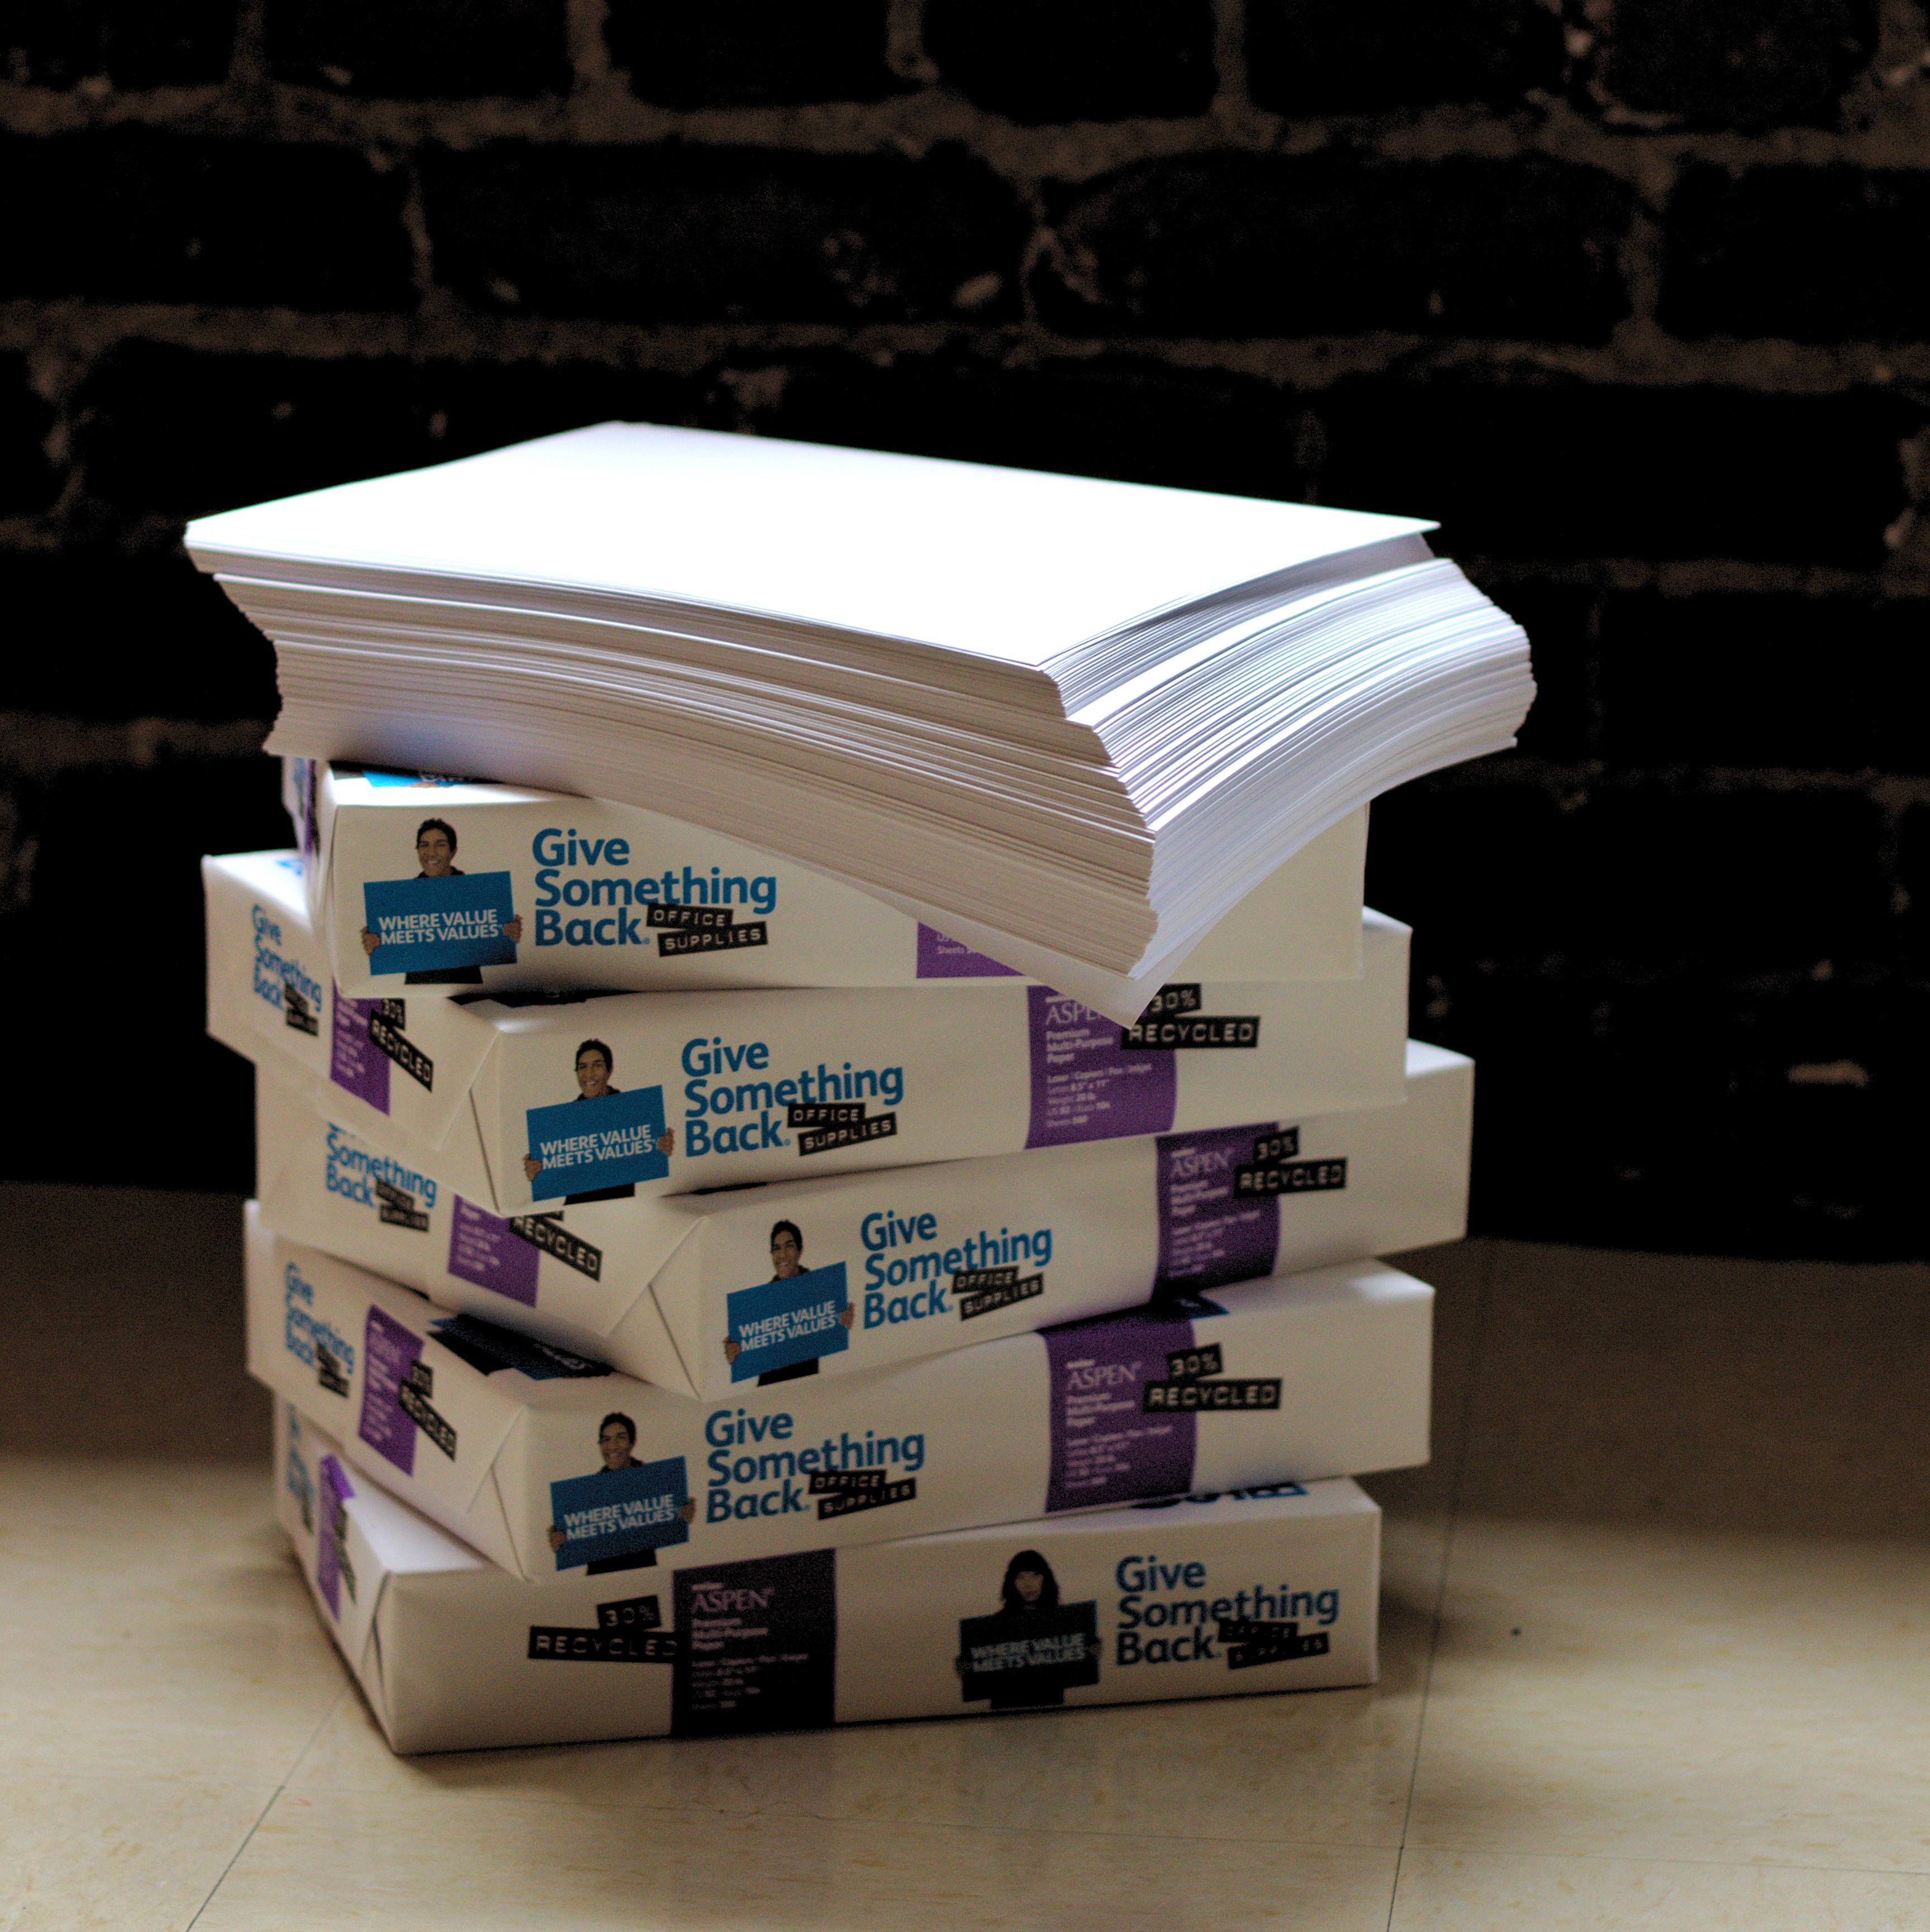
\includegraphics[width=5cm, height=4.3cm]{chapter7/figure14}} node[rotate=90, font=\tiny] at ([yshift=.5cm,xshift=.1cm]a.south east) {\textsuperscript{\textcopyright} wikipedia} ;
\node[text width=5cm] at ([yshift=0.2cm]a.north) {\mytriangle{red}{\small A ream of paper contains 500 sheets}};
 
 \node (b) at (6cm,0) {\includegraphics[width=5cm, height=4.3cm]{chapter7/figure13}} node[rotate=90, font=\tiny] at ([yshift=.5cm,xshift=.1cm]b.south east) {\textsuperscript{\textcopyright} www.wallpaperflare.com} ;
\node[text width=4cm] at ([yshift=0.2cm]b.north) {\mytriangle{red}{\small A six-pack contains 6 beers}};

 \node (c) at (12cm,.5cm) {\includegraphics[width=4.5cm, height=4.7cm]{chapter7/figure15}} node[rotate=90, font=\tiny] at ([yshift=.5cm,xshift=.1cm]c.south east) {\textsuperscript{\textcopyright} Flickr} ;
\node[text width=4cm] at ([yshift=0.2cm]c.north) {\mytriangle{red}{\small A gross is a dozen of dozens}};
\end{tikzpicture}
}
\caption{Collections of items and their name}
\label{fig:moleFig2}
\end{figure*}

For example: how many molecules are there in 3 mol of \ce{H2O}? In order to calculate the number of molecules of \ce{H2O} in 3 moles of \ce{H2O}, (moles $\rightarrow$ molecules) you need to set up a conversion factor, starting by the give information (3 moles) and using the mol-to-molecule conversion factor with mol on the bottom:
\begin{equation*}
3   \cancel{\text{moles of }\ce{H2O}} \times 
\dfrac{6.02\times 10^{23} \text{ molecules of \ce{H2O}}   } {  1\cancel{\text{mol of }\ce{H2O}}} =1.80\times 10^{24}\text{molecules of \ce{H2O} }
\end{equation*}
In you need to convert molecules to moles (molecules $\rightarrow$ moles), you just need to follow the same procedure, using the conversion factor between mol-to-molecule with molecule in the bottom. For example $3\times 10^{20}$ \ce{H2O} molecules equals to $4.98\times 10^{-4}\text{moles of \ce{H2O}}$ as
\begin{equation*}
3\times 10^{20}   \cancel{\text{molecules of }\ce{H2O}} \times 
\dfrac{ 1 \text{moles of }\ce{H2O}   } {  6.02\times 10^{23} \cancel{\text{molecules of }\ce{H2O}}} =4.98\times 10^{-4}\text{moles of \ce{H2O}}
\end{equation*}
\item[\docfilehook{From molecules to atoms}{From  molecules to atoms}] Molecules are made of atoms, and for example the \ce{CO2} molecule contains an atom of \ce{C} and two atoms of \ce{O}. In order to convert from molecules to atoms (molecules $\rightarrow$ atoms) you need to use the coefficients in the molecular formula. For example, and \ce{H2O} molecule contains an atom of \ce{O} and two atoms of \ce{H}, and hence the relation between water molecules and H and O atoms is:
\begin{equation*}
\boxed{   \frac{1\text{ molecule of  \ce{H2O} }}{1 \text{ atom of \ce{O} } }\ \text{ and  } \frac{1 \text{ molecule of \ce{H2O}}}{2 \text{ atom of \ce{H} } }\     }
\end{equation*}
To convert from moles into atoms (moles $\rightarrow$ atoms) you need to use a two-step process in a single line. First you convert from moles  into molecules, to then convert molecules into atoms. For example, 3 moles of \ce{H2O} contains $1.6\times 10^{24}$ \ce{H} atoms, as:
 \begin{equation*}\begin{split}
3   \cancel{\text{moles of }\ce{H2O}} \times 
\dfrac{6.02\times 10^{23} \cancel{\text{ molecules of \ce{H2O} }}  } {  1\cancel{\text{moles of }\ce{H2O}}} 
\times\dfrac{2 \text{H atoms}}{1\cancel{\text{ molecules of \ce{H2O} }}}
\\=1.6\times 10^{24}\text{atoms of H}
\end{split}\end{equation*}



\begin{example} %%%%%%%%%%%%%%%%%%%%%%%% EXAMPLE BOX
Calculate: (a) the number of CuO molecules in 3.4 moles of \ce{CuO}; (b) the number of moles of CO in $5\times 10^{20}$ \ce{CO} molecules; (c) The number of O atoms in 4.5 moles of \ce{NO2}. \\
\textlcsc{ \textcolor{dgreen}{\Large \textbf{Solution}} }\\
(a) 3.4 moles of \ce{CuO} equals to $2.05\times 10^{22}$ molecules of CuO as:
\begin{equation*}\begin{split}
3.4   \cancel{\text{moles of }\ce{CuO}} \times
\dfrac{6.022\times 10^{23} \text{ molecules of \ce{CuO} }  } {  1\cancel{\text{mole of  }\ce{CuO}}}=\\
=2.05\times 10^{22} \text{molecules of CuO}
\end{split}\end{equation*}
(b) $5\times 10^{20}$ \ce{CO} molecules equals to $8.3\times 10^{-4}$ moles of \ce{CO}, as
\begin{equation*}
5\times 10^{20}   \cancel{\text{CO molecules}} \times
\dfrac{ 1\text{ mole of CO}  } { 6.022\times 10^{23} \cancel{\text{ CO molecules}}   }
=8.3\times 10^{-4} \text{moles of CO}
\end{equation*}
(c) 4.5 moles of \ce{NO2} contains $5.4\times 10^{24}$ O atoms, as
 \begin{equation*}\begin{split}
4.5  \cancel{\text{moles of }\ce{NO2}} \times 
\dfrac{6.022\times 10^{23} \cancel{\ce{NO2} \text{ molecules}}  } {  1\cancel{\text{moles of }\ce{NO2}}} 
\times\dfrac{2 \text{O atoms}}{1\cancel{\ce{NO2} \text{ molecules}}}\\
=5.4\times 10^{24}\text{O atoms}
\end{split}\end{equation*}\\
\faDiamond\ \textlcsc{ \textcolor{dgreen}{\Large \textbf{Study Check}} }\\
The chemical formula for caffeine is \ce{C8H10N4O2}. Calculate the number of C, H, N and O atoms in 3.5 moles of caffeine. \\
\flushright Answer: $3.4\times 10^{25}$ moles of C, $4.2\times 10^{25}$ moles of H, $1.7\times 10^{25}$ moles of N and $8.4\times 10^{24}$ moles of O.
\end{example}%%%%%%%%%%%%%%%%%%%%%%%% EXAMPLE BOX


\end{description}
	

   \begin{marginfigure}[-9cm]
   \begin{tikzpicture} \node (a) at (0,0) {\includegraphics[width=4cm, height=4cm]{chapter7/figure5}} node[rotate=90, font=\tiny] at ([yshift=.5cm,xshift=.1cm]a.south east) {\textsuperscript{\textcopyright} www.wallpaperflare.com} ;
\node[text width=5cm] at ([yshift=0.6cm]a.north) {\mytriangle{red}The molecular mass of cinnamic acid (\ce{C9H8O2}), used in the manufacture of flavors, is $148.16 \frac{g}{mol}$ };
\end{tikzpicture}
\begin{tikzpicture} \node (a) at (0,0) {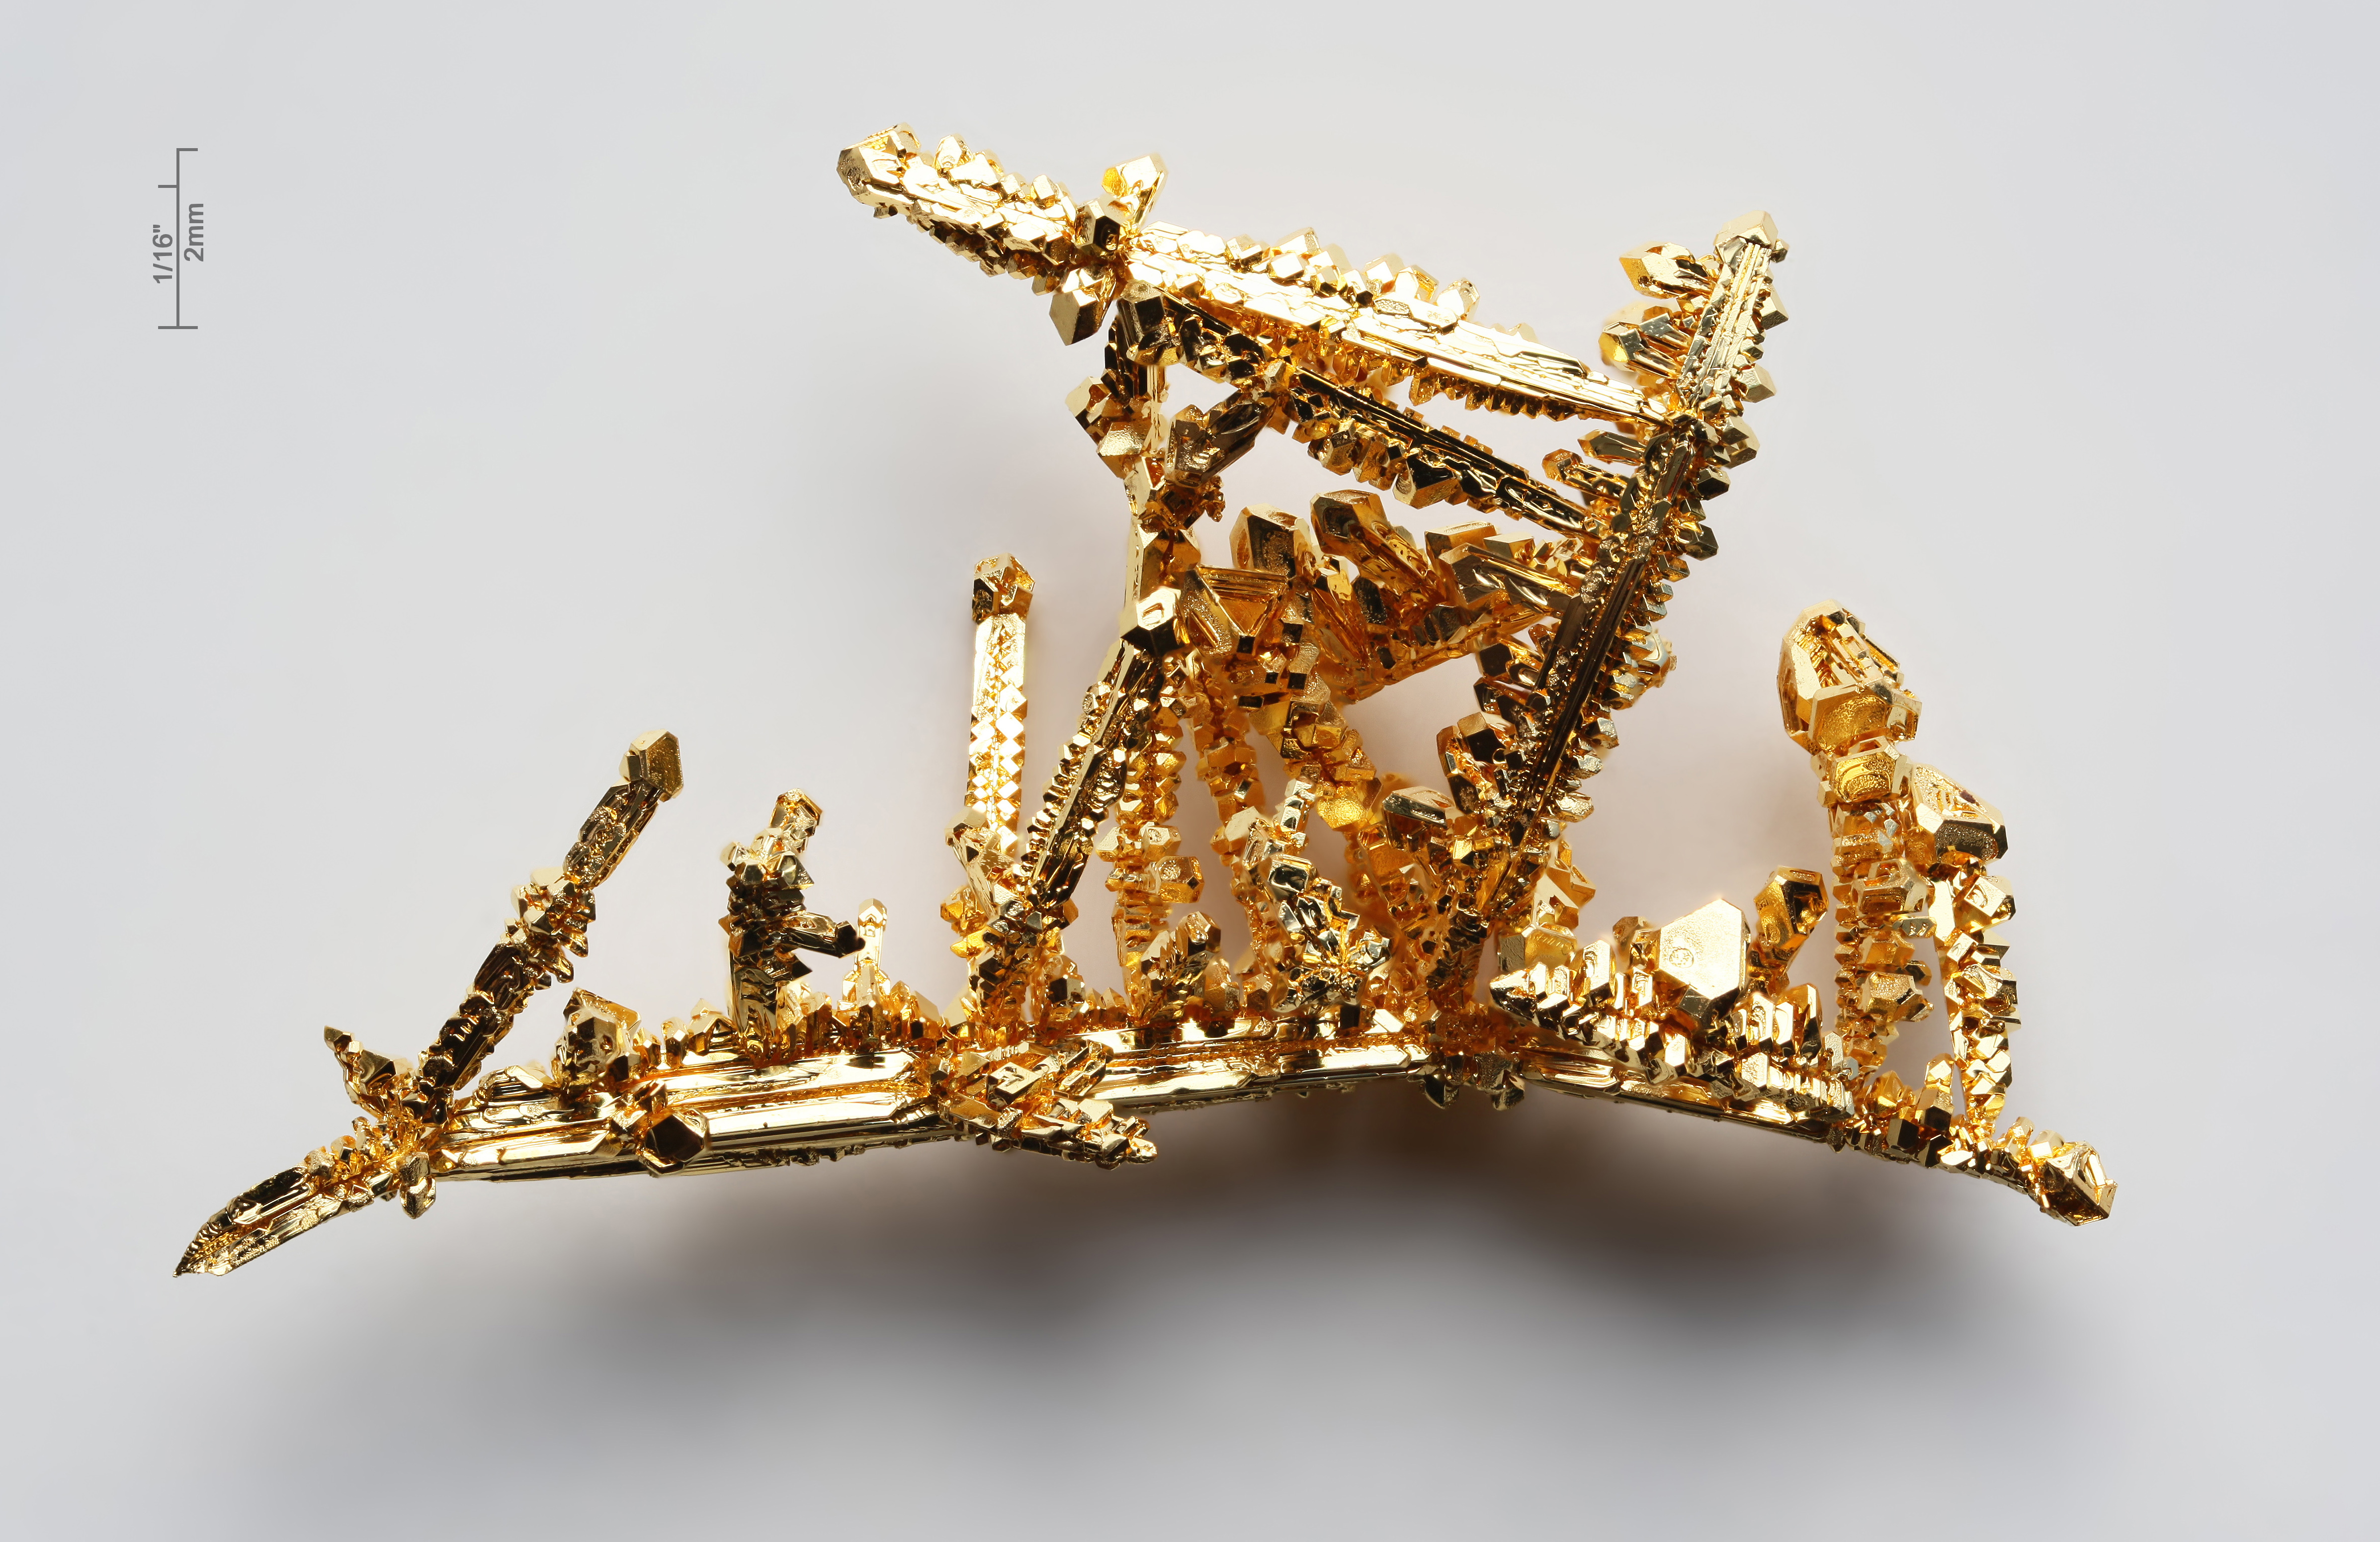
\includegraphics[width=4cm, height=4cm]{chapter7/figure6}} node[rotate=90, font=\tiny] at ([yshift=.5cm,xshift=.1cm]a.south east) {\textsuperscript{\textcopyright} www.wallpaperflare.com} ;
\node[text width=5cm] at ([yshift=0.6cm]a.north) {\mytriangle{red}Car batteries contains sulfuric acid (\ce{H2SO4}), a corrosive chemical with a molar mass of $180.06 \frac{g}{mol}$};
\end{tikzpicture}
\begin{tikzpicture} \node (a) at (0,0) {\includegraphics[width=4cm, height=4cm]{chapter7/figure7}} node[rotate=90, font=\tiny] at ([yshift=.5cm,xshift=.1cm]a.south east) {\textsuperscript{\textcopyright} wikipedia} ;
\node[text width=5cm] at ([yshift=0.6cm]a.north) {\mytriangle{red}Ammonia smelling salts (\ce{(NH4)2CO3}, MW=$96g/mol$) were historically employed to wake up injured athlete during a sport game.};
\end{tikzpicture}
\begin{tikzpicture} \node (a) at (0,0) {\includegraphics[width=4cm, height=4cm]{chapter7/figure16}} node[rotate=90, font=\tiny] at ([yshift=.5cm,xshift=.1cm]a.south east) {\textsuperscript{\textcopyright} PngImg} ;
\node[text width=5cm] at ([yshift=0.6cm]a.north) {\mytriangle{red}Acetic acid is an organic acid with molar mass $60g/mol$ };
\end{tikzpicture}
%\begin{tikzpicture} \node (a) at (0,0) {\includegraphics[width=4cm, height=6cm ]{chapter7/figure17}} node[rotate=90, font=\tiny] at ([yshift=.5cm,xshift=.1cm]a.south east) {\textsuperscript{\textcopyright} www.weberscientific.com} ;
%\node[text width=5cm] at ([yshift=0.6cm]a.north) {\mytriangle{red}Aspirin is an anti-inflammatory drug with molar mass of $180g/mol$ };
%\end{tikzpicture}
\caption{Examples of measuring equipment}
\label{fig:molFig3}
\end{marginfigure}



\section{Converting moles into grams and into atoms}
A standard way to measure chemicals in the lab is by weight. We can weight different quantities and the larger the quantity the larger the weight. For a chemical, the weigh of a mole is called the molar (or molecular) weight. For example if we weight a mole of water (\ce{H2O}) we will be weighting 18 grams of water, or if you weight a mole of table salt (\ce{NaCl}) the scale will show 58 grams. In this section you will learn how to calculate the molar mass of a chemical and how to use this property to convert from weight to moles (and moles to weight).
\sloppy 
\begin{description}
\item[\docfilehook{Molar mass of a chemical}{Molar mass of a chemical}] Chemicals are made of atoms, and each atom has an specific atomic weight (AW) listed in the periodic table. For example, the atomic weight of Na is 23 grams whereas the atomic weight of Cl is 35 g. The weight of all the atoms of a molecule is called the molecular weight (we call this also molar weight or MW). For example, the molecular weight of NaCl is 58 g, as the weight of Na and Cl is 23 and 35g. Another example would be water, \ce{H2O} with a molecular weight of 18g--as the atomic weight of H and O is 1 and 16 g, respectively, and the molecule has two H atoms. The units for molecular weight is $\frac{g}{mol}$, also written as $g/mol$. In order to compute the molar mass of a molecule you need to break down the molecule into atoms using the coefficients in the formula. For example, the formula for vinegar is \ce{C2H4O2} that means a vinegar molecule contains 2C, 4H and 2O atoms. If you add the atomic masses of 2C, 4H and 2O you will get $60g/mol$. If the chemical formula has a parenthesis, you need to open up the parenthesis to calculate the total number of atoms. As an example, \ce{Ca(NO3)2} contains 1Ca, 2N, and 6O, and its molar mass is $164.09g/mol$.

\begin{example} %%%%%%%%%%%%%%%%%%%%%%%% EXAMPLE BOX
Calculate: (a) The atomic weight of Mg; (b) the molecular mass of sulfuric acid, \ce{H2SO4} \\
\textlcsc{ \textcolor{dgreen}{\Large \textbf{Solution}} }\\
(a) According to the periodic table the atomic weight (AW) of Mg is $24.31g/mol$. (b) The molar mass of \ce{H2SO4} is the result of adding the atomic masses of 2H (AW=$1g/mol$) atoms, 1 S (AW=$32g/mol$) and 4O (AW=$16g/mol$)  atoms, that gives $98.08g/mol$.\\
\faDiamond\ \textlcsc{ \textcolor{dgreen}{\Large \textbf{Study Check}} }\\
Calculate the molar mass of glucose \ce{C6H12O6}\\
\flushright Answer: $180.06g/mol$.
\end{example}%%%%%%%%%%%%%%%%%%%%%%%% EXAMPLE BOX



\item[\docfilehook{From moles to grams}{From moles to grams}] The molar mass is used to convert moles to grams or grams to mol. For example, the molar mass of water is $18 g/mol$. This means:
\begin{equation*}
\boxed{   1 \text{mole of \ce{H2O}}=18 \text{g of \ce{H2O}}   } 
\end{equation*}
that is the same as
\begin{equation*}
\boxed{   \frac{\text{1 mole of \ce{H2O} }}{ \text{18 grams of } \ce{H2O}}\ \text{ or  } \frac{ \text{18 grams of }\ce{H2O} }{\text{1 mole of \ce{H2O}}}\     }
\end{equation*}

\begin{figure}
    \centering
    \resizebox{.9\textwidth}{6cm}{
\begin{tikzpicture}[
   planet/.style = {circle, draw=blue, semithick, fill=blue!30,
                    font=\large\bfseries, 
                    text width=24mm, inner sep=1mm,align=center}, %<---
satellite/.style = {circle, draw=#1, semithick, fill=#1!30,
                    text width=16mm, inner sep=1mm, align=center},%<---
      arr/.style = {-{Triangle[length=3mm,width=6mm]}, color=#1,
                    line width=3mm, shorten <=1mm, shorten >=1mm}
                    ]
\node (p)   [planet]    {1 mole};
\foreach \i/\j [count=\k] in {red/{18 g \ce{H2O}}, cyan/{{\small $6.02\times 10^{23}$} molecules of \ce{H2O}}, purple/{{\small $6.02\times 10^{23}$} molecules of \ce{CO2}}, teal/{{\small $6.02\times 10^{23}$} molecules of \ce{NH3}}, orange/{17 g \ce{NH3}}, yellow/{44 g \ce{CO2}}}
{
    \node (s\k) [satellite=\i] at (\k*60:3.4) {\j};
    \draw[arr=\i] (p) -- (s\k);
}
    \end{tikzpicture}}
\caption{A mole is equivalent to the same number of molecules for different chemicals. Differently, a mole is equivalent to different weights of different chemicals.}
\end{figure}






\begin{example} %%%%%%%%%%%%%%%%%%%%%%%% EXAMPLE BOX
Smelling salts (\ce{(NH4)2CO3}) are chemical used to arouse consciousness. These are used by pro athletes to get into the zone before a game.  How many moles of salt do you have in 100 grams of these salts? \\
\textlcsc{ \textcolor{dgreen}{\Large \textbf{Solution}} }\\
We first need to calculate the molar mass of \ce{(NH4)2CO3}, a chemical with 2N, 8H, 1C and 3O atoms. The molar mass hence would be: $2\times 5+8\times 1+1\times 12 + 3\times 16=96g/mol$. In order to calculate the moles given the gram, you need to use the molar mass a conversion factor:
 \begin{equation*}
100  \cancel{\text{g of \ce{(NH4)2CO3}}} \times 
\dfrac{\text{moles of }\ce{(NH4)2CO3} } { \cancel{96\text{ g of \ce{(NH4)2CO3}}} } 
=\text{1.04 moles of }\ce{(NH4)2CO3}
\end{equation*}\\
\faDiamond\ \textlcsc{ \textcolor{dgreen}{\Large \textbf{Study Check}} }\\
Calculate the MW of table salt (\ce{NaCl}) and the grams in 20 moles of this salt. \\
\flushright Answer: $58.4g/mol$; 1168g.
\end{example}%%%%%%%%%%%%%%%%%%%%%%%% EXAMPLE BOX

%\begin{marginfigure}%%%%%%%MARGIN FIGURE
%      \includegraphics{chapter7/figure12}
%      \caption{1 gram of S contains $1.8\times 10^{22}$ atoms}
%	\end{marginfigure}%%%%%%%MARGIN FIGURE

\item[\docfilehook{From grams to atoms}{From grams to atoms}] In the previous sections we covered how to convert grams to moles, and moles to molecules, or molecules to atoms. You can follow the diagram below in order to switch from one of these properties (atoms, molecules, moles, grams) to another.\\

\begin{tikzpicture}
\node [block] (box1) at (0,0) [rectangle,draw=white,fill=red!20!white] {\textcolor{blue}{Grams of \ce{H2O}}};
\node [block] (box2) at  (3,0) [rectangle,draw=white,fill=orange!20!white] {\textcolor{blue}{Moles of \ce{H2O}}};
\node [block] (box3) at  (7,0) [rectangle,draw=white,fill=yellow!20!white] {\textcolor{blue}{Molecules of \ce{H2O}}};
\node [block] (box4) at  (10,0) [rectangle,draw=white,fill=green!20!white] {\textcolor{blue}{Atoms of H}};
\node [block] (box5) at  (3,4) [rectangle,draw=white,fill=green!20!white] {\textcolor{blue}{Moles of H}};
\draw[thick,->] (box1.east) -- (box2.west) node[above,pos=0.5] {MW} node[below=0.3cm,pos=0.5] { $\frac{\text{1 mole of }\ce{H2O}}{18\text{ g of }\ce{H2O}}$};


\draw[thick,->] (box2.east) -- (box3.west) node[above,pos=0.5] {Avogadro's \#}node[below=0.3cm,pos=0.5] {$\frac{\text{1 mole of }\ce{H2O}}{6.02\times 10^{23}\text{ molecules of }\ce{H2O}}$};
\draw[thick,->] (box3.east) -- (box4.west) node[above,pos=0.5] {Formula}node[below=0.3cm,pos=0.5] {$\frac{\text{1 molecule of }\ce{H2O}}{2\text{ atoms of H}}$};
\draw[thick,->] (box2.north) -- ++(0,1) -- ++(7,0) node[below,pos=0.5] {\ce{H2O} moles to H atoms} -- (box4.north);
\draw[thick,->] ([xshift=-0.5cm]box2.north) -- ++(0,3)  node[below,pos=0.5, rotate=90, yshift=1.15cm, text width=3cm,xshift=0.25cm] {moles of \ce{H2O} to moles of \ce{H} } node[right=0.3cm,pos=0.5, text width=3cm, yshift=0.5cm, xshift=-0.25cm] {$\frac{\text{1 mole of }\ce{H2O}}{2\text{ moles of H}}$};
\draw[thick,->] (box1.south) -- ++(0,-1)  -- ++(10,0)  node[below,pos=0.5] {\ce{H2O} grams to H atoms} -- (box4.south);
\end{tikzpicture}


For example, if you want to convert grams into moles, you will only need one step and you will only have to use a single property: the molar mass. Differently, if you need to convert grams into molecules you will have to use two different steps and use two different properties: the molar mass and Avogadro's number.

\begin{example} %%%%%%%%%%%%%%%%%%%%%%%% EXAMPLE BOX
Convert 10 grams of ammonia (\ce{NH3}, MW=$17g/mol$) into H atoms.\\
\textlcsc{ \textcolor{dgreen}{\Large \textbf{Solution}} }\\
We will have to do this conversion in three different steps. First we will go from grams to moles, then from moles to molecules to finally transform molecules into atoms:
 \begin{equation*}\begin{split}
10  \cancel{\text{g of \ce{NH3}}} \times 
\dfrac{\text{1 mole of \ce{NH3}} } { \cancel{\text{17 g of \ce{NH3}}} } \times
\dfrac{6.022\times 10^{23}\text{ \ce{NH3} molecules} }{\cancel{\text{1 mole of \ce{NH3}}}} \times \\
\dfrac{\text{3 H atoms} } { \cancel{\text{1 \ce{NH3} molecule}} } =1.8\times 10^{24}\text{H atoms}
\end{split}\end{equation*}\\
\faDiamond\ \textlcsc{ \textcolor{dgreen}{\Large \textbf{Study Check}} }\\
Methane is a chemical used as a fuel. Calculate how many grams of methane \ce{CH4} contains $5\times 10^{25}$ H atoms. \\
\flushright Answer: 332.1g.
\end{example}%%%%%%%%%%%%%%%%%%%%%%%% EXAMPLE BOX
\end{description}



   \begin{marginfigure}[0cm]
   \begin{tikzpicture} \node (a) at (0,0) {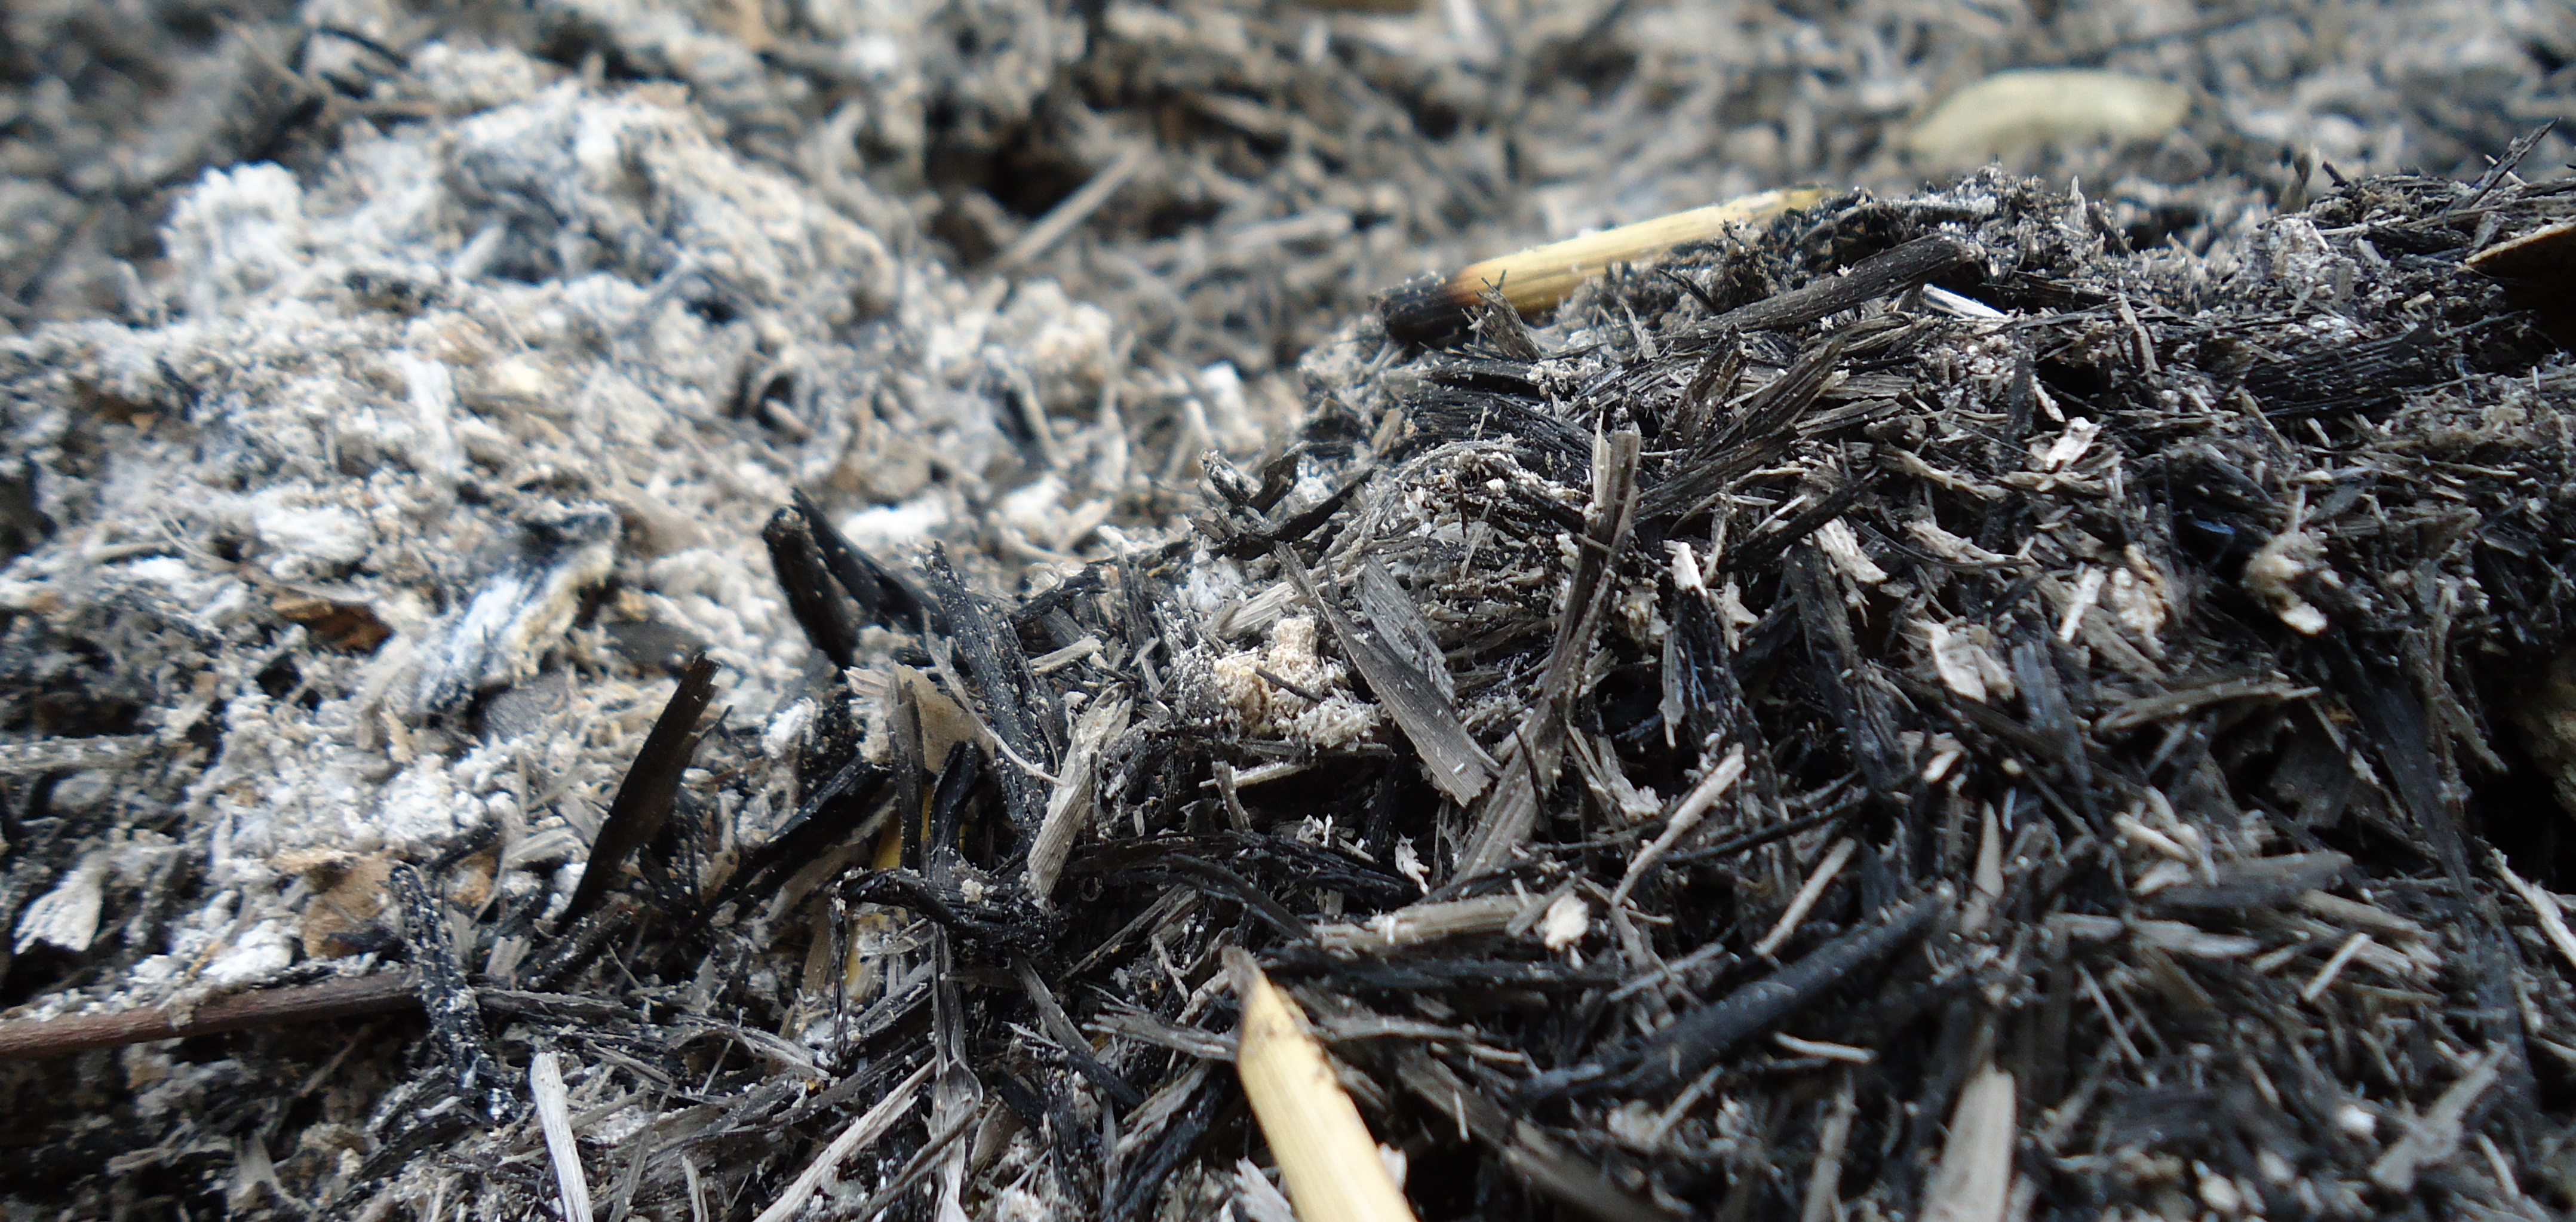
\includegraphics[width=4cm, height=4cm]{chapter7/figure8}} node[rotate=90, font=\tiny] at ([yshift=.5cm,xshift=.1cm]a.south east) {\textsuperscript{\textcopyright} www.wallpaperflare.com} ;
\node[text width=5cm] at ([yshift=0.6cm]a.north) {\mytriangle{red}A termite reaction between iron(III) oxide and Al: \ce{Fe2O3 + 2Al -> 2Fe + Al2O3} };
\end{tikzpicture}
\begin{tikzpicture} \node (a) at (0,0) {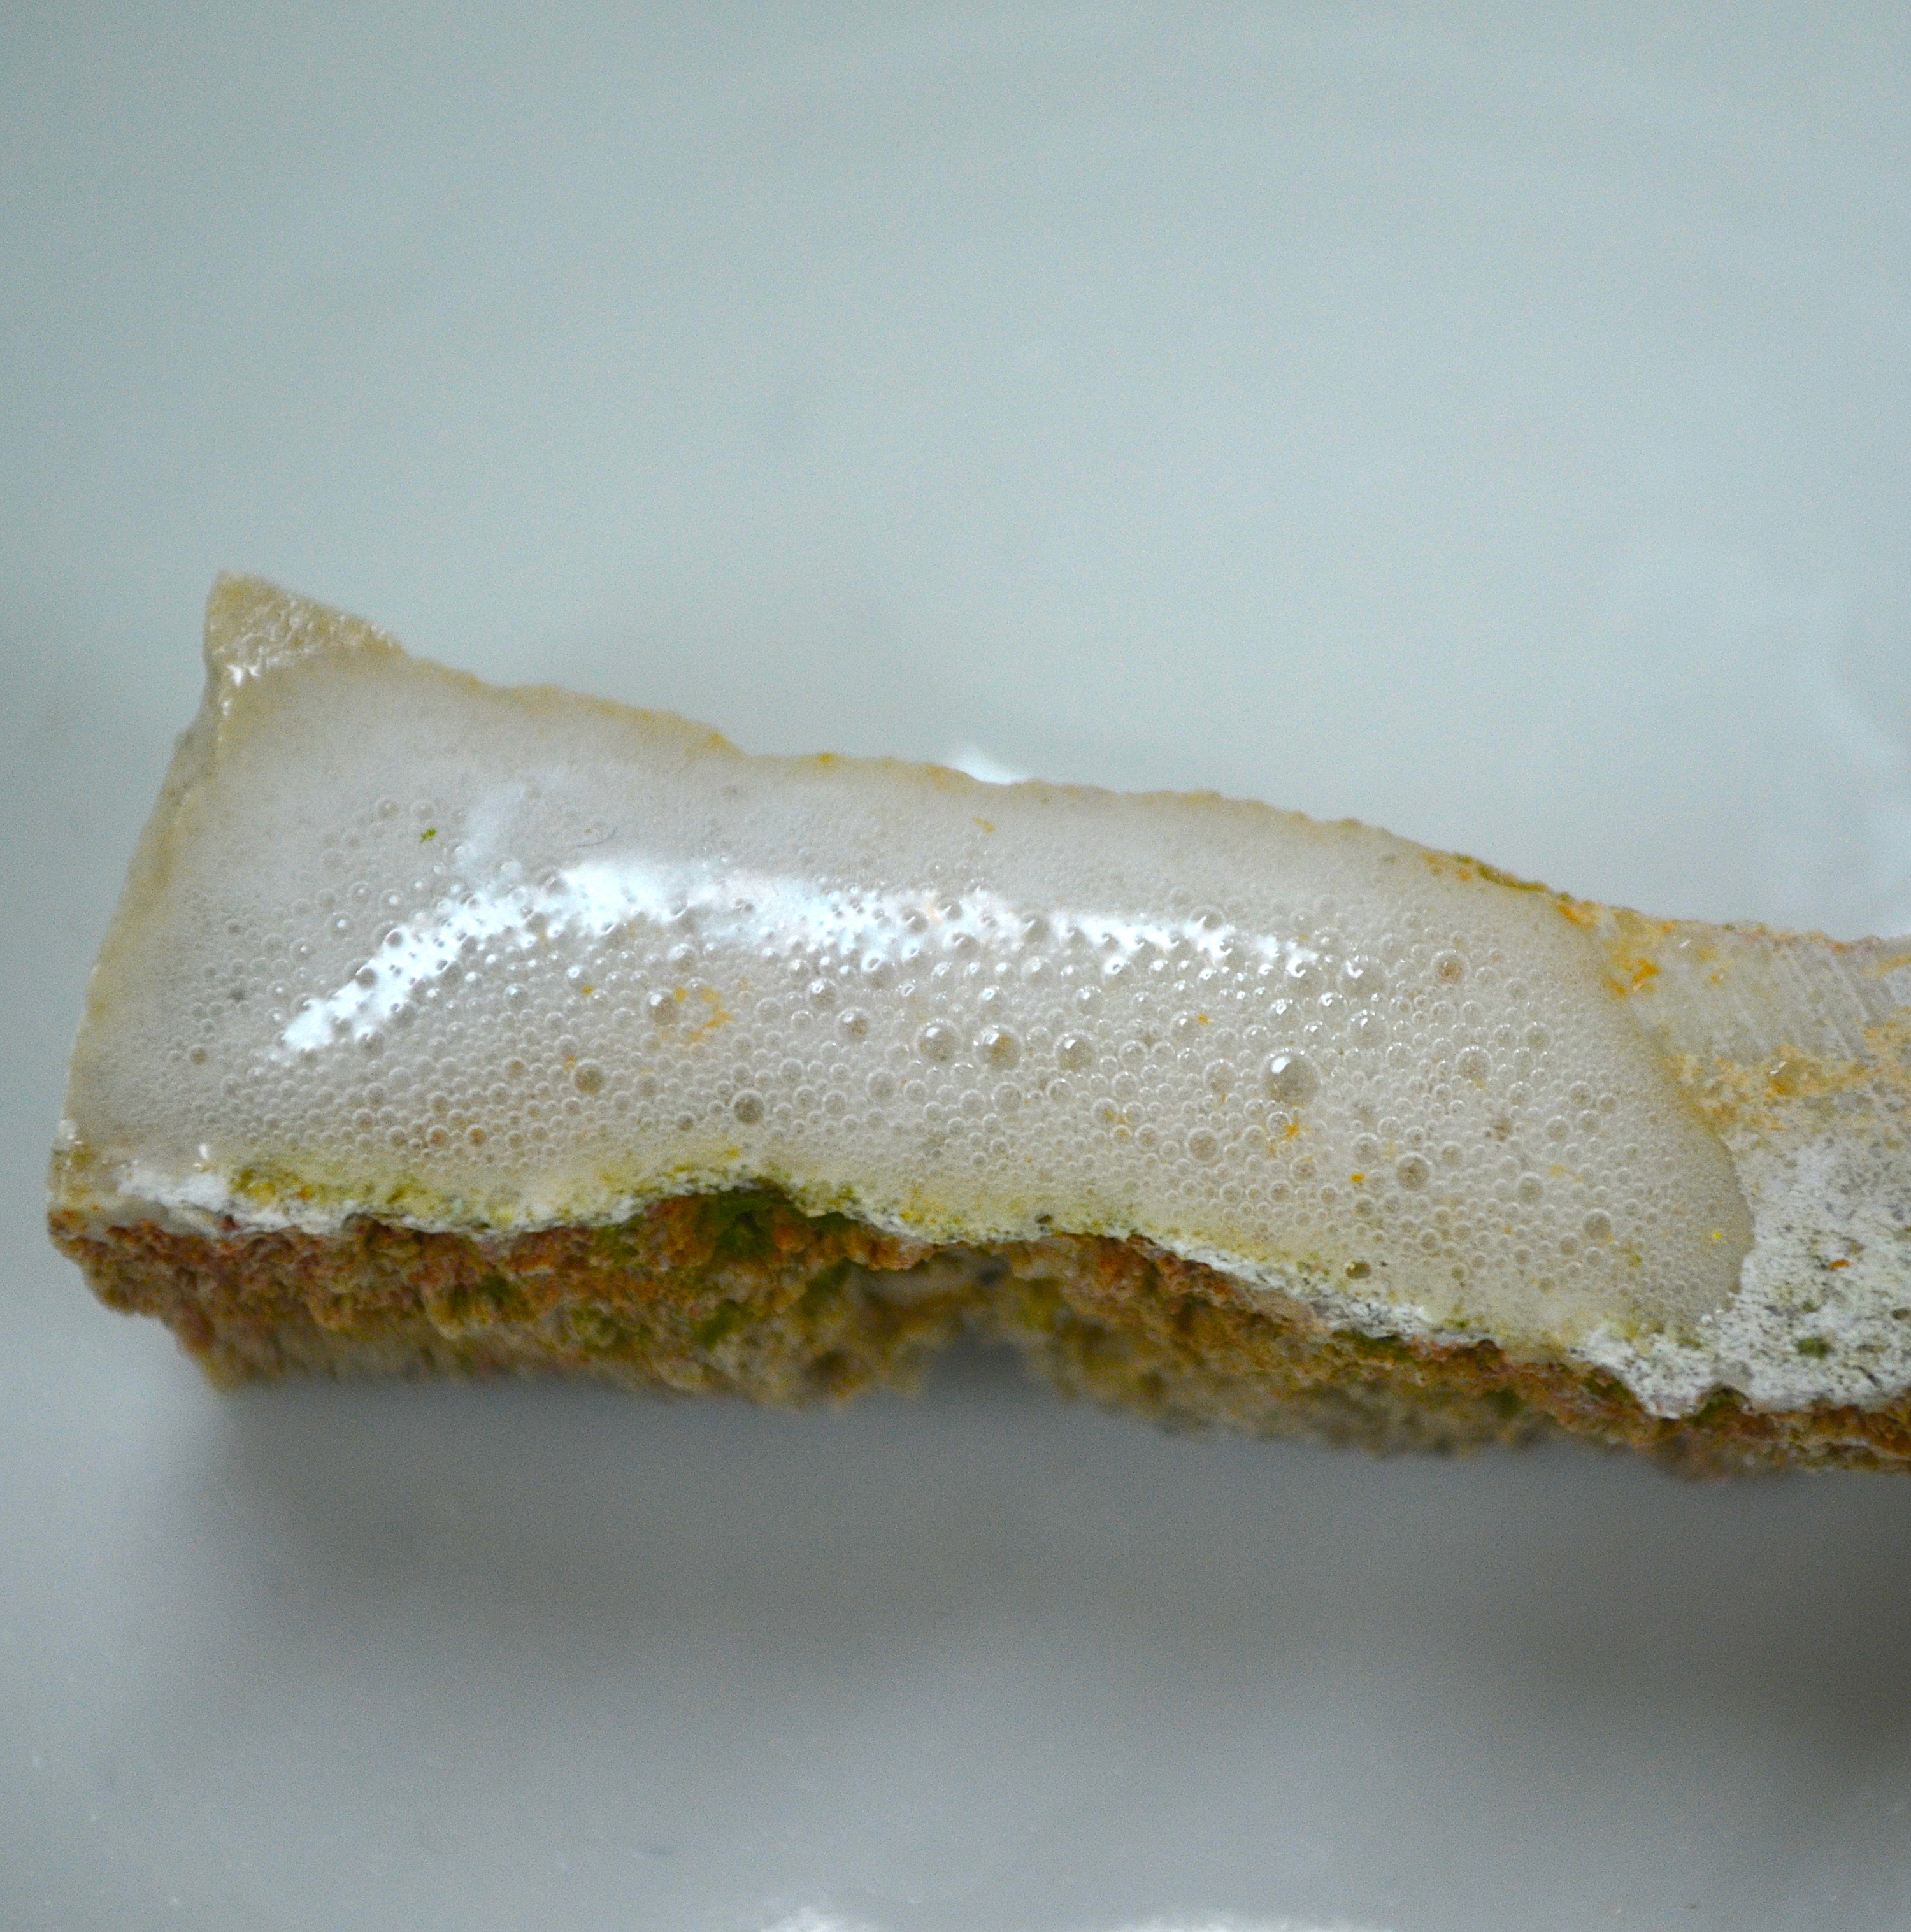
\includegraphics[width=4cm, height=4cm]{chapter7/figure11}} node[rotate=90, font=\tiny] at ([yshift=.5cm,xshift=.1cm]a.south east) {\textsuperscript{\textcopyright} www.wallpaperflare.com} ;
\node[text width=5cm] at ([yshift=0.6cm]a.north) {\mytriangle{red}An image of the combustion of Mg: \ce{2Mg(s) + O2(g) -> 2MgO(s)}};
\end{tikzpicture}
\begin{tikzpicture} \node (a) at (0,0) {\includegraphics[width=4cm, height=4cm]{chapter7/figure9}} node[rotate=90, font=\tiny] at ([yshift=.5cm,xshift=.1cm]a.south east) {\textsuperscript{\textcopyright} wikipedia} ;
\node[text width=5cm] at ([yshift=0.6cm]a.north) {\mytriangle{red}Iron rust is the result of a combination reaction: \ce{4Fe + 2O2 -> 2Fe2O3}};
\end{tikzpicture}
\begin{tikzpicture} \node (a) at (0,0) {\includegraphics[width=4cm, height=4cm]{chapter7/figure10}} node[rotate=90, font=\tiny] at ([yshift=.5cm,xshift=.1cm]a.south east) {\textsuperscript{\textcopyright} PngImg} ;
\node[text width=5cm] at ([yshift=0.6cm]a.north) {\mytriangle{red}Wood burning is a combustion reaction };
\end{tikzpicture}
%\begin{tikzpicture} \node (a) at (0,0) {\includegraphics[width=4cm, height=6cm ]{chapter7/figure17}} node[rotate=90, font=\tiny] at ([yshift=.5cm,xshift=.1cm]a.south east) {\textsuperscript{\textcopyright} www.weberscientific.com} ;
%\node[text width=5cm] at ([yshift=0.6cm]a.north) {\mytriangle{red}Aspirin is an anti-inflammatory drug with molar mass of $180g/mol$ };
%\end{tikzpicture}
\caption{Examples of reactions}
\label{fig:molFig4}
\end{marginfigure}
\section{Chemical reactions}
When we eat we burn food with molecular oxygen (\ce{O2}) to produce carbon dioxide and water. Similarly, when we start the engine of the car to go to work, gasoline burns to produce the same chemicals: \ce{CO2} and \ce{H2O}. These are two examples of chemical reactions, but there are many other examples. Nitrogen from the air reacts with hydrogen to produce ammonia, a common chemical used in the production of fertilizers. This section covers the basic of chemical reactions. You will learn how to balance reaction and how classify reactions.
\sloppy 



\begin{description}
\item[\docfilehook{Simple chemical reactions}{Simple chemical reactions}] Magnesium is a metal that react with oxygen to produce magnesium oxide. Magnesium is solid \ce{Mg_{(s)}} whereas oxygen is gas and contains two oxygen atoms per molecule \ce{O2_{(g)}}. Magnesium oxide, the result of the reaction, is solid \ce{MgO_{(s)}}. The reaction between magnesium and oxygen to produce magnesium oxide
\begin{center}\ce{2Mg_{(s)} + 1O2_{(g)} -> 2MgO_{(s)}}\end{center}
\ce{Mg} and \ce{O2} combine together--that is why we use a plus sign-- to produce \ce{MgO}--we use an arrow to indicate that a chemical is being produced. Also the symbols \begin{it}(s)\end{it} or \begin{it}(g)\end{it} indicates solid or gas state. The reactants are located before the arrow and the products after the arrow. The numbers in front of the reactants and products (2,1 and 2) are called stoichiometric coefficients, and we will talk more about them in the following sections.
\item[\docfilehook{Reading a chemical reaction}{Reading chemical reactions}]
Chemicals reactions can be read in words. In order to read a chemical reaction you need to connect the reactants with the word \say{react} and then use the words \say{to produce} and after that you need to read the products. The numbers in front of the reactants and products represent the number of moles, and you need to include those numbers in the reading. For example, the following reaction
\begin{center}\ce{2Mg(s) + O2(g) -> 2MgO(s)}\end{center}
should be read as: \say{two moles of Mg react with one mole of \ce{O2} to produce two moles of \ce{MgO}}. 

\item[\docfilehook{Balanced chemical reactions}{Balanced chemical reactions}]
Chemical reactions contain molecules, which are made of atoms. Some chemical reactions are balanced, and others need to be balanced. In order to identify a balanced reaction, you should use the stoichiometric coefficients and the indexes in the molecular formulas to break down the reactants and products into atoms. In a balanced chemical reaction, the atoms of reactants should be the same as the atoms of the products. Consider the following reaction, \\
\begin{center}\ce{2Mg(s) + O2(g) -> 2MgO(s)}.\end{center}
The table below shows all reactants and products in the form of atoms. 
\begin{tabularx}{\linewidth}{XXX}
\toprule
\multicolumn{3}{c}{\ce{2Mg(s) + O2(g) -> 2MgO(s)} } \tabularnewline
\toprule
\multicolumn{1}{l}{   \textcolor{cyan}{Reactants} }& \textcolor{cyan}{Products} & \tabularnewline
\toprule
  2Mg &  2Mg  &\checkmark \tabularnewline
    \ce{O2}=2O &  2O &\checkmark \tabularnewline
\bottomrule
\end{tabularx}
The number of Mg atoms in the reactants and products is the same, and equals to two. On the other hand, the number of O atoms in the reactants and products is the same, being equal to two. For this reason, we say this reaction is \emph{balanced}.\\
Now consider the following reaction:
\begin{center}\ce{C(s) + O2(g) -> CO(g)},\end{center}
The number of C atoms in the reactants and products is the same, and equals to one. In contrast, the number of O atoms in the reactants and products is not the same, and for this reason, we say this reaction is \emph{not balanced}.
\begin{tabularx}{\linewidth}{XXX}
\toprule
\multicolumn{3}{c}{\ce{C(s) + O2(g) -> CO(g)} } \tabularnewline
\toprule
\multicolumn{1}{l}{   \textcolor{cyan}{Reactants} }& \textcolor{cyan}{Products} & \tabularnewline
\toprule
 1C &  1C  &\checkmark \tabularnewline
  \ce{O2}=2O &  O & \xmark \tabularnewline
\bottomrule
\end{tabularx}
 


\item[\docfilehook{Balancing chemical reactions}{Balancing chemical reactions}]
In order to balance a reaction, we need to introduce the stoichiometric coeficientes that make the number of atoms of reactants and products the same. In order to balance the number of oxygens, we will multiply \ce{CO} by two, and that will give us two oxygens and two carbons as well. If we do this, now the carbon atoms of reactants and products will not be the same. We can solve this by multiplying \ce{C(s)} by two. The following table summarizes the changes we made:
\begin{tabularx}{\linewidth}{XXX}
\toprule
\multicolumn{3}{c}{\ce{2C(s) + O2(g) -> 2CO(g)} } \tabularnewline
\toprule
\multicolumn{1}{l}{   \textcolor{cyan}{Reactants} }& \textcolor{cyan}{Products} & \tabularnewline
\toprule
 2C &  2C  &\checkmark \tabularnewline
    \ce{O2}=2O &  2O &\checkmark  \tabularnewline
\bottomrule
\end{tabularx}
The reaction is now balanced after introducing  two stoichiometric coefficients and the number of C and O atoms in the reactant molecules and products is the same.



\begin{example} %%%%%%%%%%%%%%%%%%%%%%%% EXAMPLE BOX
Balance the following reaction:
\begin{center}\ce{CH4(g) + O2(g) -> CO2(g) + H2O(g)}\end{center}
\textlcsc{ \textcolor{dgreen}{\Large \textbf{Solution}} }\\
We will break down each molecule into atoms. In the case of O, both \ce{CO2} and \ce{H2O} contain oxygen and hence you will have to combine both oxygen atoms:
\begin{tabularx}{\linewidth}{XXX}%% REACTION TABLE
\toprule
\multicolumn{3}{c}{\ce{CH4(g) + O2(g) -> CO2(g) + H2O(g)} } \tabularnewline
\toprule
\multicolumn{1}{l}{   \textcolor{cyan}{Reactants} }& \multicolumn{1}{l}{ \textcolor{cyan}{Products}} & \tabularnewline
\toprule
1C &  1C  &\checkmark \tabularnewline
  4H &   2H  &\xmark \tabularnewline
 2O &    3O  &\xmark \tabularnewline
\bottomrule
\end{tabularx}%% REACTION TABLE

The reaction is not balanced as the number of H and O atoms for the reactants and products is not the same. In order to balance the H, you can multiply by two \ce{H2O}, and that will balance H but also affect  O.\\
\begin{tabularx}{\linewidth}{XXX}%% REACTION TABLE
\toprule
\multicolumn{3}{c}{\ce{CH4(g) + O2(g) -> CO2(g) + 2H2O(g)} } \tabularnewline
\toprule
\multicolumn{1}{l}{   \textcolor{cyan}{Reactants} }& \multicolumn{1}{l}{ \textcolor{cyan}{Products}} & \tabularnewline
\toprule
1C &  1C  &\checkmark \tabularnewline
  4H &   4H  &\checkmark \tabularnewline
 2O &    4O  &\xmark \tabularnewline
\bottomrule
\end{tabularx}%% REACTION TABLE
\\
You can balance O by multiplying \ce{O2} by two. That will give you the final balanced reaction in which all atoms (O, H and C) are the same in the product and reactant molecules.
\\
\begin{tabularx}{\linewidth}{XXX}%% REACTION TABLE
\toprule
\multicolumn{3}{c}{\ce{CH4(g) + 2O2(g) -> CO2(g) + 2H2O(g)} } \tabularnewline
\toprule
\multicolumn{1}{l}{   \textcolor{cyan}{Reactants} }& \multicolumn{1}{l}{ \textcolor{cyan}{Products}} & \tabularnewline
\toprule
1C &  1C  &\checkmark \tabularnewline
  4H &   4H  &\checkmark \tabularnewline
 4O &    4O  &\checkmark \tabularnewline
\bottomrule
\end{tabularx}%% REACTION TABLE
\vspace{0.5cm}
\faDiamond\ \textlcsc{ \textcolor{dgreen}{\Large \textbf{Study Check}} }\\
Balance the following reaction: \ce{Fe2O3(s) + C(s) -> Fe(s) + CO(g)}
\flushright Answer: \ce{Fe2O3(s) + 3C(s) -> 2Fe(s) + 3CO(g)}.\\
\end{example}%%%%%%%%%%%%%%%%%%%%%%%% EXAMPLE BOX


\item[\docfilehook{Five types of reactions}{Five types of reactions}]
Most of the chemical reactions can be classified according to five types: combination, decomposition, single replacement, double replacement and combustion. \\
In a \emph{combinations reaction} two reactants combine to generate a product. An example of a combination is the reaction between Mg and oxygen to produce \ce{MgO}:
\begin{center}\ce{2Mg(s) + O2(g) -> 2MgO(s) \textcolor{red}{ (combination)}}\end{center}
In a \emph{decomposition reaction} a single reactant breaks down into several products. An example of a decomposition reaction is the thermal reaction of \ce{CaCO3} to produce calcium oxide (\ce{CaO}) and carbon dioxide
\begin{center}\ce{CaCO3(s) -> CaO(s) + CO2(g) \textcolor{red}{ (decomposition)}}\end{center}
In a single replacement reaction, an element replaces another element in a chemical. An example would be the reaction of Zn with \ce{HCl}, in which Zn replaces hydrogen:
\begin{center}\ce{\textcolor{blue}{Zn}(s) + 2HCl(aq) -> \textcolor{blue}{Zn}Cl2(aq) + H2(g) \textcolor{red}{ (Single replacement)}}\end{center}
In a double replacement reaction, the first element in the reacting compounds switch places. An example is the reaction between \ce{AgNO3} and \ce{NaCl}, in which Ag from \ce{AgNO3} replaces Na in \ce{NaCl}:
\begin{center}\ce{\textcolor{blue}{Ag}NO3(aq) + \textcolor{green}{Na}Cl(aq) ->  \textcolor{green}{Na}NO3(aq) + \textcolor{blue}{Ag}Cl(s) \textcolor{red}{ (Double replacement)}}\end{center}
Finally, in a combustion reaction, a carbon-based chemical reacts with oxygen to produce carbon dioxide and water. An example would be the combustion of methane (\ce{CH4}):
\begin{center}\ce{CH4(g) + 2O2(g) -> 2H2O(g) + CO2(g) \textcolor{red}{ (Combustion)}}\end{center}





\end{description}



\section{Stoichiometry and mass calculations}
In the previous section, you learned how to balance a chemical reaction. In order to do this, you had to find the stoichiometric coefficients that balance the atoms of the reactant and products. In this new section we will learn how to use those coefficients to predict the amount of product formed. You will also learn how to predict the amount of reactant needed to react with another reactant. We will use the reaction between Mg and oxygen:
\begin{center}\ce{2Mg(s) + O2(g) -> 2MgO(s)}\end{center}
in which two moles of Mg and one mole of \ce{O2} produce two moles of \ce{MgO}. We will refer to this reaction in the following.
\sloppy 
\begin{description}
\item[\docfilehook{Mole-Mole ratio}{Mole-Mole ratio}] 
Chemical reaction can be expressed in the form of conversion factors. 
For example, the mole ratio between Mg (a reactant) and \ce{O2} (another reactant) and between Mg and \ce{MgO} is:
\begin{equation*}
\boxed{   \frac{\text{2 moles of Mg}}{\text{1 moles of } \ce{O2}}\ \text{ or  } \frac{ \text{1 moles of } \ce{O2}}{ \text{2 moles of Mg}}\ \text{ and }\: \frac{\text{2 moles of Mg}}{\text{2 moles of } \ce{MgO}}\ \text{ or  } \frac{ \text{2 moles of } \ce{MgO}}{ \text{2 moles of Mg}}\   }
\end{equation*}

Finally, the mole ratio between \ce{O2} and \ce{MgO} is:
\begin{equation*}
\boxed{   \frac{\text{1 moles of }\ce{O2}}{\text{2 moles of } \ce{MgO}}\ \text{ or  } \frac{ \text{2 moles of } \ce{MgO}}{ \text{1 moles of }\ce{O2}}\   }
\end{equation*}
Mole ratios are used, for example, to transform the amount of reactant into product.
\item[\docfilehook{Reactants to products}{Reactants to products}] 
We will calculate how much MgO will be produced from 5 moles of Mg by converting Mg into MgO by means of the conversion factor between both chemicals. As we want to transform the Mg into MgO we will use the conversion factor with Mg on the bottom of the fraction. This way the units will cancel out to give moles of MgO:
 \begin{equation*}
5\cancel{\text{ moles of Mg}} \times \dfrac{\text{2 moles of MgO}}{2\cancel{\text{ moles of Mg}}}=5\text{ moles of MgO}.
\end{equation*}
This result means that 5 moles of Mg will produce 5 moles of MgO.

\item[\docfilehook{Reactant to a different reactant}{Reactant to a different reactant}] 
Sometimes we will have to calculate how much reactant will be needed to react with another reactant. In those cases we will use the conversion factor that relates both reactants. If we have 5 moles of Mg and we want to know how much oxygen do we need to react with Mg, we will proceed as:
\begin{equation*}
5\cancel{\text{ moles of Mg}} \times \dfrac{\text{1 mole of }\ce{O2}}{2\cancel{\text{ moles of Mg}}}=2.5\text{ moles of }\ce{O2}.
\end{equation*}
This result means that 2.5 moles of \ce{O2} will react with 5 moles of Mg.

\begin{example} %%%%%%%%%%%%%%%%%%%%%%%% EXAMPLE BOX
Hydrogen reacts with oxygen to produce water according to the following reaction
\begin{center}\ce{2H2(g) + O2(g) -> 2H2O(g)}\end{center}
Calculate: (a) the number of moles of water produced from 5 moles of \ce{H2}; (b) the number of moles of oxygen needed to react with 7 moles of \ce{H2}.\\
\textlcsc{ \textcolor{dgreen}{\Large \textbf{Solution}} }\\
(a) we will first convert 5 moles of \ce{H2} into water:
\begin{equation*}
5\cancel{\text{ moles of }\ce{H2}} \times \dfrac{\text{2 moles of }\ce{H2O}}{2\cancel{\text{ moles of }\ce{H2}}}=5\text{ moles of }\ce{H2O},
\end{equation*}
that is: 5 moles of hydrogen produce 5 moles of water.
(b) We will now calculate the amount of oxygen needed to react with 7 moles of hydrogen
\begin{equation*}
7\cancel{\text{ moles of }\ce{H2}} \times \dfrac{\text{1 moles of }\ce{O2}}{2\cancel{\text{ moles of }\ce{H2}}}=3.5\text{ moles of }\ce{O2},
\end{equation*}
that is: 3.5 moles of \ce{O2} will react with 7 moles of \ce{H2}.
\\
\faDiamond\ \textlcsc{ \textcolor{dgreen}{\Large \textbf{Study Check}} }\\
Calculate the number of moles of water produced by 4 moles of oxygen. \\
\flushright Answer: 8 moles.
\end{example}%%%%%%%%%%%%%%%%%%%%%%%% EXAMPLE BOX

\item[\docfilehook{Mass calculations}{Mass calculations}] 
In the previous sections, given the moles of reactants, we learned how to use chemical reactions to predict the amount of product formed. In this section we will learn how to do the same, but instead of starting with the number of moles, this time, we will work our way starting with a quantity given in grams. We will based the following examples in the reaction of Mg and \ce{O2}:
\begin{center}\ce{2Mg(s) + O2(g) -> 2MgO(s)}\end{center}
\item[\docfilehook{Molar mass review}{Molar mass review}] 
Remember that the molar mass (also known as molecular weight, MW. Atomic weight for the atoms, AW) of a chemical is a property used to convert grams into moles. For example the molar mass of \ce{H2O} is $18g/mol$. If we need to convert 12 grams of water into mols we should do:
 \begin{equation*}
12  \cancel{\text{g of \ce{H2O}}} \times 
\dfrac{\text{moles of \ce{H2O} }} { 18\cancel{\text{ g of \ce{H2O}}} } 
=\text{0.66 moles of \ce{H2O}}
\end{equation*}
In order to use the stoichiometric coefficients from a chemical reaction, the starting quantity must be the moles of a reactant of products. This is because these coefficients are expressed in moles and hence in order to operate with them you can only use moles. 
\item[\docfilehook{Grams to moles in a reaction}{Grams to moles in a reaction}] 
If we want to calculate the grams of MgO produced from 3 moles of Mg, we will start with the moles of Mg and use a conversion factor that relates moles of Mg and moles of MgO, locating the moles of Mg on the bottom:
\begin{equation*}
3\cancel{\text{ moles of }\ce{Mg}} \times \dfrac{\text{2 moles of }\ce{MgO}}{2\cancel{\text{ moles of }\ce{Mg}}}=3\text{ moles of }\ce{MgO}.
\end{equation*}
Now we aim to calculate the number of MgO moles produced from 5 grams of Mg (AW=$24g/mol$). This times, we will have first to convert the grams of Mg into moles to then use the mole ration between Mg and MgO:
\begin{equation*}
5\cancel{\text{ g of }\ce{Mg}}   \times  \dfrac{1 \cancel{\text{ moles of }\ce{Mg}}}{24\cancel{\text{ g of }\ce{Mg}}}
 \times \dfrac{\text{2 moles of }\ce{MgO}}{2\cancel{\text{ moles of }\ce{Mg}}}=0.21\text{ moles of }\ce{MgO}.
\end{equation*}

\item[\docfilehook{Grams to grams in a reaction}{Grams to grams in a reaction}] 
We want to answer the following question: we have 6 moles of Mg (AW=$24g/mol$) and we want to calculate the mass of MgO(MW=$40g/mol$) produced. The importance of this type of calculations is based on the fact that in a chemistry laboratory chemicals are normally weighted in grams. In order to answer this example, we will start with the grams of Mg and convert this quantity to moles of Mg using the atomic mass. After that we will use the mole ratio between Mg and MgO to calculate the moles of MgO. Aft this point, we will finish the calculation by converting the moles of MgO into grams using its molecular weight:

\begin{equation*}\begin{split}
5\cancel{\text{ grams of }\ce{Mg}}   \times  \dfrac{1 \cancel{\text{ moles of }\ce{Mg}}}{24\cancel{\text{ grams of }\ce{Mg}}}
 \times \dfrac{2\cancel{\text{ moles of }\ce{MgO}}}{2\cancel{\text{ moles of }\ce{Mg}}}
  \times  \dfrac{40\text{ grams of }\ce{MgO}}{1\cancel{\text{ moles of }\ce{MgO}}}\\
 =10\text{ grams of }\ce{MgO}.
\end{split}\end{equation*}
Overall, we have that 5 grams of Mg will produce 10 grams of MgO.

\begin{example} %%%%%%%%%%%%%%%%%%%%%%%% EXAMPLE BOX
For the reaction of hydrogen and nitrogen to produce ammonia (\ce{NH3}):
\begin{center}\ce{3H2(g) + N2(g) -> 2NH3(g) } \end{center}
Calculate: (a) the number of moles of \ce{NH3}  produced from 10 grams of hydrogen (MW=$2g/mol$); (b) Calculate the number of grams of \ce{NH3} (MW=$17g/mol$) produced from 10 grams of nitrogen (MW=$28g/mol$) \\
\textlcsc{ \textcolor{dgreen}{\Large \textbf{Solution}} }\\
(a) You will solve this problem in a single line by using two steps: first convert the grams of hydrogen to moles, to then convert the moles of hydrogen into ammonia:
\begin{equation*}
10\cancel{\text{ grams of }\ce{H2}}   \times  \dfrac{1\cancel{\text{ moles of }\ce{H2}}}{2\cancel{\text{ grams of }\ce{H2}}}
 \times \dfrac{\text{2 moles of }\ce{NH3}}{3\cancel{\text{ moles of }\ce{H2}}}=3.33\text{ moles of }\ce{NH3}.
\end{equation*}
In other words, 10 grams of hydrogen produce 3.33 moles of ammonia. (b) To solve this question, we will use one additional step in order to convert the moles of ammonia into grams:
\begin{equation*}\begin{split}
10\cancel{\text{ grams of }\ce{N2}}   \times  \dfrac{1\cancel{\text{ moles of }\ce{N2}}}{28\cancel{\text{ grams of }\ce{N2}}}
 \times \dfrac{2\cancel{\text{ moles of }\ce{NH3}}}{1\cancel{\text{ moles of }\ce{N2}}}
  \times  \dfrac{17\text{ grams of }\ce{NH3}}{1\cancel{\text{ moles of }\ce{NH3}}}\\
 =12.14\text{ grams of }\ce{NH3}.
\end{split}\end{equation*}
\\
\faDiamond\ \textlcsc{ \textcolor{dgreen}{\Large \textbf{Study Check}} }\\
Calculate the number of grams of nitrogen needed to react with 3 grams of hydrogen to produce ammonia. \\
\flushright Answer: 14 grams.
\end{example}%%%%%%%%%%%%%%%%%%%%%%%% EXAMPLE BOX

\end{description}

 








\section{Percent yield and limiting reagent}
Often, reactions do not fully proceed to completion. Fewer amounts of products are obtained when a specific quantity of a chemical is expected from a reaction. The percent yield tells how much of the final chemical is produced. The larger the yield the larger the amount of products generated and therefore, the less waste is generated. At the same time, when mixing two reactants sometimes leftovers remain. In other words, sometimes there is a reagent that limits the reaction and an excess reagent. This section will cover the very important ideas of percent yield and limiting (or excess) reagent.
\sloppy 
\begin{description}

\item[\docfilehook{Percent yield}{Percent Yield}] 
Chemical reactions are less than perfect as staring material does not fully convert into products. Furthermore, side reactions often occur in competition with the main reaction generating byproducts. The theoretical yield is the amount of products one will expect in a hypothetically perfect chemical reaction, while the actual yield is the amount of product that is in fact produced. Therefore, the percent yield is just the fraction between the actual yield and the theoretical yield in percent form:
\begin{equation*}
 \text{Percent Yield}=\dfrac{\text{actual yield}}{\text{theoretical yield}}\times 100
\end{equation*}
To compute the percent yield, we need the theoretical yield, which is the amount of product that will be produced following the rules of stoichiometry, and the actual yield, normally known in an experiment from lab measurements.
Look at the scenario below: we need two wheels and a body to ensemble a bike. We can think about the bike production yield based on the starting materials we have. \begin{center}\vspace{1cm}\hspace{-0.5cm}\begin{tikzpicture}[x=1cm,y=1cm]
\begin{scope}[transform canvas={shift={(-7em,0em)}	},scale=0.3, every node/.append style={transform shape}]\bikewheel\end{scope}
 \begin{scope}[transform canvas={shift={(-5em,0em)}	},scale=0.3, every node/.append style={transform shape}]\bikewheel\end{scope}
 \begin{scope}[transform canvas={shift={(0em,0)}	},scale=0.3, every node/.append style={transform shape}]{\bikebody} \end{scope}
\begin{scope}[transform canvas={shift={(12em,0em)}	},scale=1.0, every node/.append style={transform shape}] \draw [->, thick] (-2,0) -- (-1,0);\end{scope}
\begin{scope}[transform canvas={shift={(12em,0em)}	},scale=0.3, every node/.append style={transform shape}]{\bike}\end{scope}
\end{tikzpicture}\end{center}
If we have three pairs of wheels and three bodies and we only produce two bikes, the yield will be $67\%$. 
\begin{center}\vspace{1cm}\begin{tikzpicture}[x=1cm,y=1cm]
\begin{scope}[transform canvas={shift={(-15em,0em)}	},scale=0.3, every node/.append style={transform shape}]\bikewheel\end{scope}
\begin{scope}[transform canvas={shift={(-13em,0em)}	},scale=0.3, every node/.append style={transform shape}]\bikewheel\end{scope}
\begin{scope}[transform canvas={shift={(-11em,0em)}	},scale=0.3, every node/.append style={transform shape}]\bikewheel\end{scope}
\begin{scope}[transform canvas={shift={(-9em,0em)}	},scale=0.3, every node/.append style={transform shape}]\bikewheel\end{scope}
\begin{scope}[transform canvas={shift={(-7em,0em)}	},scale=0.3, every node/.append style={transform shape}]\bikewheel\end{scope}
 \begin{scope}[transform canvas={shift={(-5em,0em)}	},scale=0.3, every node/.append style={transform shape}]\bikewheel\end{scope}
 \begin{scope}[transform canvas={shift={(-1em,2em)}	},scale=0.3, every node/.append style={transform shape}]{\bikebody} \end{scope}
 \begin{scope}[transform canvas={shift={(0em,0)}	},scale=0.3, every node/.append style={transform shape}]{\bikebody} \end{scope}
 \begin{scope}[transform canvas={shift={(1em,-2em)}	},scale=0.3, every node/.append style={transform shape}]{\bikebody} \end{scope}
\begin{scope}[transform canvas={shift={(12em,0em)}	},scale=1.0, every node/.append style={transform shape}] \draw [->, thick] (-2,0) -- (-1,0);\end{scope}
\begin{scope}[transform canvas={shift={(12em,0em)}	},scale=0.3, every node/.append style={transform shape}]{\bike}\end{scope}
\begin{scope}[transform canvas={shift={(14em,-2em)}	},scale=0.3, every node/.append style={transform shape}]{\bike}\end{scope}
\end{tikzpicture}\end{center}\vspace{1cm}
\begin{example} %%%%%%%%%%%%%%%%%%%%%%%% EXAMPLE BOX
Ammonia is produced by reacting molecular nitrogen and molecular hydrogen following the reaction:
\begin{center}\ce{3H2_{(g)} + N2_{(g)} -> 2NH3_{(g)} } \end{center}
What is the percent yield of ammonia if 4 moles of hydrogen gives 2 moles of ammonia.  \\
\textlcsc{ \textcolor{dgreen}{\Large \textbf{Solution}} }\\
We will first compute the theoretical yield, that is the moles of ammonia produced from 4 moles of hydrogen:
\begin{equation*}
4\cancel{\text{ moles of }\ce{H2}} \times \dfrac{\text{2 moles of }\ce{NH3}}{3\cancel{\text{ moles of }\ce{H2}}}=2.66\text{ moles of }\ce{NH3}.
\end{equation*}
Hence the theoretical yield is 2.66 moles of \ce{NH3}, and the actual yield given in the problem is 2 moles of \ce{NH3}. The actual yield is smaller than the theoretical yield. That is reasonable as the moles of ammonia produced in the real experiment should always be smaller than the amount of ammonia produced in theory. To calculate the percent yield we use the formula:
\begin{equation*}
 \text{Percent Yield}=\dfrac{\text{actual yield}}{\text{theoretical yield}}\times 100=\frac{2}{2.66}\times 100=75.18\%
\end{equation*}
\\
\faDiamond\ \textlcsc{ \textcolor{dgreen}{\Large \textbf{Study Check}} }\\
Calculate the percent yield of ammonia if 1 moles of nitrogen gives 1.5 moles of ammonia \\
\flushright Answer: $75\%$.
\end{example}%%%%%%%%%%%%%%%%%%%%%%%% EXAMPLE BOX


\item[\docfilehook{Limiting reagent}{Limiting reagent}] 
Let us consider the reaction between solid carbon and molecular oxygen to produce \ce{CO2}:
\begin{center}\ce{C_{(s)} + O2_{(g)} -> CO2_{(g)} } \end{center}
This reaction should be read as \say{one mole of carbon reacts with one mole of molecular oxygen to produce one mole of carbon dioxide}. Mind that to produce one mole of \ce{CO2} you need one mole of C and one mole of molecular oxygen. Now, what would happen if you mix one mole of carbon with 0.5 moles of oxygen? In this scenario, when the 0.5 moles of oxygen are consumed the reaction will stop; half a mole of carbon dioxide will be formed and half a mole of C will remain. Differently, no oxygen will remain and the whole 0.5 moles will consume. We say that C is the excess reactant and oxygen the limiting reactant. 

Often times a reaction will be accompanied with the reagent quantities and you will have to identify the limiting reagent. This reagent will limit the amount of product formed, and hence, any stoichiometric calculation aimed to predict the amount of product formed should be based on the limiting reagent and never on the excess reagent.  Next we will explain how to systematically identify the limiting reagent.
\item[\docfilehook{Identifying the limiting reagent}{Identifying the limiting reagent}] 
Consider the following reaction, in which 3 moles of Mg react with 2 moles of oxygen to produce magnesium oxide:
\begin{center}  \ce{ $\underset{\text{3 moles}}{\ce{2Mg}}$ + $\underset{\text{2 moles}}{\ce{O2}}$ -> 2MgO }\end{center}
In order to identify the limiting reagent, we will chose one of the given reagent quantities and calculate the moles of the other reagent needed  (we will call this $n_{needed}$). For example, if we choose to start with 3 moles of Mg, the amount of oxygen needed to react with this quantity will be:
\begin{equation*}
n_{needed}^{\ce{O2}}=3\cancel{\text{ moles of }\ce{Mg}} \times \dfrac{\text{1 moles of }\ce{O2}}{2\cancel{\text{ moles of }\ce{Mg}}}=1.5\text{ moles of }\ce{O2}.
\end{equation*}
This means that to react with 3 moles of Mg you need $n_{needed}^{\ce{O2}}=1.5$ moles of oxygen. On the other hand, you have two moles of oxygen ($n_{given}^{\ce{O2}}=2$), and that is more than what you need to react with the 3 moles of Mg. Hence, 
\begin{equation*}
n_{needed}^{\ce{O2}}<n_{given}^{\ce{O2}}
\end{equation*}
oxygen is the excess reagent and Mg the limiting reagent. The left overs will be:
\begin{equation*}
n_{left}^{\ce{O2}}= \abs*{ n_{needed}^{\ce{O2}}-n_{given}^{\ce{O2}} }=0.5 \text{ moles of }\ce{O2}
\end{equation*}
Let us reinforce the idea of limiting reagent with the scenario below. If we have three  wheels and two bodies, the number of wheels limits the bike production. 
\begin{center}\vspace{1cm}\begin{tikzpicture}[x=1cm,y=1cm]
%\begin{scope}[transform canvas={shift={(-15em,0em)}	},scale=0.3, every node/.append style={transform shape}]\bikewheel\end{scope}
%\begin{scope}[transform canvas={shift={(-13em,0em)}	},scale=0.3, every node/.append style={transform shape}]\bikewheel\end{scope}
\begin{scope}[transform canvas={shift={(-11em,0em)}	},scale=0.3, every node/.append style={transform shape}]\bikewheel\end{scope}
\begin{scope}[transform canvas={shift={(-9em,0em)}	},scale=0.3, every node/.append style={transform shape}]\bikewheel\end{scope}
\begin{scope}[transform canvas={shift={(-7em,0em)}	},scale=0.3, every node/.append style={transform shape}]\bikewheel\end{scope}
% \begin{scope}[transform canvas={shift={(-5em,0em)}	},scale=0.3, every node/.append style={transform shape}]\bikewheel\end{scope}
 \begin{scope}[transform canvas={shift={(-1em,2em)}	},scale=0.3, every node/.append style={transform shape}]{\bikebody} \end{scope}
 \begin{scope}[transform canvas={shift={(0em,0)}	},scale=0.3, every node/.append style={transform shape}]{\bikebody} \end{scope}
 %\begin{scope}[transform canvas={shift={(1em,-2em)}	},scale=0.3, every node/.append style={transform shape}]{\bikebody} \end{scope}
\begin{scope}[transform canvas={shift={(12em,0em)}	},scale=1.0, every node/.append style={transform shape}] \draw [->, thick] (-2,0) -- (-1,0);\end{scope}
\begin{scope}[transform canvas={shift={(12em,0em)}	},scale=0.3, every node/.append style={transform shape}]{\bike}\end{scope}
%\begin{scope}[transform canvas={shift={(14em,-2em)}	},scale=0.3, every node/.append style={transform shape}]{\bike}\end{scope}
\end{tikzpicture}\end{center}
Differently, if we have three wheels and one body, then the body of the bikes limit the production.
\begin{center}\vspace{1cm}\begin{tikzpicture}[x=1cm,y=1cm]
%\begin{scope}[transform canvas={shift={(-15em,0em)}	},scale=0.3, every node/.append style={transform shape}]\bikewheel\end{scope}
%\begin{scope}[transform canvas={shift={(-13em,0em)}	},scale=0.3, every node/.append style={transform shape}]\bikewheel\end{scope}
\begin{scope}[transform canvas={shift={(-11em,0em)}	},scale=0.3, every node/.append style={transform shape}]\bikewheel\end{scope}
\begin{scope}[transform canvas={shift={(-9em,0em)}	},scale=0.3, every node/.append style={transform shape}]\bikewheel\end{scope}
\begin{scope}[transform canvas={shift={(-7em,0em)}	},scale=0.3, every node/.append style={transform shape}]\bikewheel\end{scope}
% \begin{scope}[transform canvas={shift={(-5em,0em)}	},scale=0.3, every node/.append style={transform shape}]\bikewheel\end{scope}
% \begin{scope}[transform canvas={shift={(-1em,2em)}	},scale=0.3, every node/.append style={transform shape}]{\bikebody} \end{scope}
 \begin{scope}[transform canvas={shift={(0em,0)}	},scale=0.3, every node/.append style={transform shape}]{\bikebody} \end{scope}
 %\begin{scope}[transform canvas={shift={(1em,-2em)}	},scale=0.3, every node/.append style={transform shape}]{\bikebody} \end{scope}
\begin{scope}[transform canvas={shift={(12em,0em)}	},scale=1.0, every node/.append style={transform shape}] \draw [->, thick] (-2,0) -- (-1,0);\end{scope}
\begin{scope}[transform canvas={shift={(12em,0em)}	},scale=0.3, every node/.append style={transform shape}]{\bike}\end{scope}
%\begin{scope}[transform canvas={shift={(14em,-2em)}	},scale=0.3, every node/.append style={transform shape}]{\bike}\end{scope}
\end{tikzpicture}\end{center}\vspace{1cm}

\begin{example} %%%%%%%%%%%%%%%%%%%%%%%% EXAMPLE BOX
In the synthesis of ammonia (\ce{NH3}):
\begin{center}  \ce{ $\underset{\text{2 moles}}{\ce{3H2(g)}}$ + $\underset{\text{2 moles}}{\ce{N2(g)}}$ -> 2NH3(g) }\end{center}
you mix 2 moles of hydrogen with 2 moles of nitrogen. Identify the limiting and excess reagents and indicate the moles of leftover remaining.\\
\textlcsc{ \textcolor{dgreen}{\Large \textbf{Solution}} }\\
We will choose one of the reagents, for example the two moles of hydrogen, and calculate the amount of nitrogen needed to react with this amount of oxygen:
\begin{equation*}
2\cancel{\text{ moles of }\ce{H2}} \times \dfrac{\text{1 moles of }\ce{N2}}{3\cancel{\text{ moles of }\ce{H2}}}=0.66\text{ moles of }\ce{N2}.
\end{equation*}
Therefore, to react with 2 moles of hydrogen we need 0.66 moles of nitrogen, and we have 2 moles of nitrogen. This means we have more nitrogen than what we need and hence, nitrogen is the excess reagent and hydrogen the limiting reagent. As we need 0.66 moles of nitrogen and we have 2 moles, 1.33 moles of nitrogen will remain.
\\
\faDiamond\ \textlcsc{ \textcolor{dgreen}{\Large \textbf{Study Check}} }\\
You mix 3 moles of hydrogen with 0.5 moles of nitrogen. Identify the limiting and excess reagents and indicate the moles of leftover remaining. \\
\flushright Answer: \ce{N2} is the limiting reagent and \ce{H2} the excess. 0.5 moles of hydrogen will remain.
\end{example}%%%%%%%%%%%%%%%%%%%%%%%% EXAMPLE BOX

\end{description}




\end{document}


%\textquotesingle
%\section{The atom}\marginnote{ \faEnvelope\myemail{dtorresrangel@bmcc.cuny.edu}{Error in the Book}{ Send Me typos!}}
%XXXXX
%\sloppy
%\begin{description}
%\item[\docfilehook{Elements and Symbols}{Elements and Symbols}] 
%\end{description}
%

%\begin{marginfigure}%%%%%%%QUOTES
%    \begin{shadequote}[l]{Democritus}
%Nothing exists except atoms and empty space; everything else is opinion.
%\end{shadequote}   \end{marginfigure}%%%%%%QUOTES


%\begin{marginfigure}%%%%%%%MARGIN FIGURE
%      \includegraphics{chapter2/figure1}
%      \label{fig:marginfig}
%   \end{marginfigure}%%%%%%%MARGIN FIGURE

%\begin{definition}[Political Factors]%%%%%%%%%ADITIONAL INFO BOX
%\begin{minipage}{0.25\linewidth}
%\includegraphics[width = \linewidth]{example-image-a}
%\end{minipage}%
%\hfill
%\begin{minipage}{0.7\linewidth}
%Analyses to what degree the government intervenes in the
%economy. It includes regulations and legal issues and defines
%both formal and informal rules under which the firm must
%operate. Political factors include: tax policy, employment laws,
%environmental regulations, trade restriction tariffs and political
%stability.
%\end{minipage}%
%\end{definition}%%%%%%%%%ADITIONAL INFO BOX
%
%\begin{example} %%%%%%% EXAMPLE BOX with explanation
%Obtain the electronic configuration of C.\\
%\textlcsc{ \textcolor{dgreen}{\Large Solution} }\\
%The atomic number of C is Z=6 and that means C has 6 electrons. The orbital order from Figure \ref{fig:orbitaltable} is: $1s$,$2s$, $2p$, $3s$, etc. Each $s$ orbital can fit two electrons, whereas the occupancy of  the $p$ orbitals is six electrons. Hence the electronic configuration of C is: $1s^2 2s^2 2p^2$. The $s$ orbitals are all filled, whereas the $p$ orbital is only occupied with two electrons.
%\\
%\faDiamond\ \textlcsc{ \textcolor{dgreen}{\Large \textbf{Study Check}} }\\Obtain the electronic configuration of Ni.
%\flushright Answer: $1s^2 2s^2 2p^6 3s^2 3p^6 4s^2 3d^8$. 
%\end{example}
%\begin{marginfigure}
%\begin{work} % 
%\textlcsc{ \textcolor{olive}{\Large Get the Answer by: } }
%\begin{enumerate}
%\item Get the electrons
%\item Check the orbital order table
%\item Fill each orbital following the order
%\end{enumerate}
%\end{work}% 
%\end{marginfigure}%%%%%%% EXAMPLE BOX with explanation

% \begin{marginfigure}%%%%% DISCUSSION
%\begin{tcolorbox}[enhanced,colback=red!5!white,colframe=black!50!red,boxrule=1pt,
%  arc=0pt,outer arc=0pt,drop heavy lifted shadow]
%\faGears\ 
%\docenvdef{Discussion:} Look around your apartment and list a pure substance, a compound, a heterogeneous mixture and a homogeneous mixture?\end{tcolorbox}
% \end{marginfigure} %%%%% DISCUSSION
%Table \ref{tab:units} % TABLE OR FIGURE REFERENCE




%\vspace{6mm} \begin{equation*}%%%% COMMENTED EQUATION
%    \mathcal{A} = (\,\tikzmark{identity}{\texttt{I}} -\tikzmark[red]{G}{\texttt{G}}\,\,\, 
%    \tikzmark[blue]{L}{\texttt{L}} - \tikzmark[purple]{C}{\texttt{C }}\,)
%\end{equation*}
%\begin{tikzpicture}[overlay, remember picture,node distance =1.5cm]
%    \node (identitydescr) [below left=of identity ]{words};
%    \draw[,->,thick] (identitydescr) to [in=-90,out=90] (identity);
%    \node[red] (Gdescr) [below =of G]{other words};
%    \draw[red,->,thick] (Gdescr) to [in=-90,out=90] (G);
%    \node[blue,xshift=1cm] (Ldescr) [above right =of L]{some words};
%    \draw[blue,->,thick] (Ldescr) to [in=45,out=-90] (L.north);
%    \node[purple] (Cdescr) [below right =of C]{more words};
%    \draw[purple,->,thick] (Cdescr) to [in=-90,out=90] (C.south);
%\end{tikzpicture}\vspace{10mm} %%%% COMMENTED EQUATION


%\begin{tcolorbox}[tab2,tabularx={X||Y|Y|Y|Y||Y}]%%%% FANCY COLOR TABLE
%Group & One     & Two     & Three    & Four     & Sum      \\\hline\hline
%Red   & 1000.00 & 2000.00 &  3000.00 &  4000.00 & 10000.00 \\\hline
%Green & 2000.00 & 3000.00 &  4000.00 &  5000.00 & 14000.00 \\\hline
%Blue  & 3000.00 & 4000.00 &  5000.00 &  6000.00 & 18000.00 \\\hline\hline
%Sum   & 6000.00 & 9000.00 & 12000.00 & 15000.00 & 42000.00
%\end{tcolorbox}%%%% FANCY COLOR TABLE


%\begin{center}\schemestart%%% ANNONATED CHEM EQUATION
%\chemname{\ce{H2O}}{Alcohol\\test1}
%\arrow(.mid east--.mid west)
%\chemname{\ce{H2O}}{Ester}
%\+
%\chemname{\ce{H2O}}{Ester}
%\schemestop\end{center}%%% ANNONATED CHEM EQUATION
%


%\begin{figure}[h!]%%%%% EMBEDED MOVIES
%\includemovie[
%  poster=FlashPoster.jpg,width=0.25\textwidth
%  text={\Large\bf Click to start\hspace*{400pt}}
%]{550pt}{400pt}{blendone.swf}
%\end{figure}%%%%% EMBEDED MOVIES



%\begin{marginfigure}%%%%%%%MARGIN PLOT
%\begin{tikzpicture}[yscale=0.8]
%\begin{axis}[axis background/.style = {%
%      shade,
%      top color = blue!10,
%      bottom color = white},
%    x tick label style={
%        /pgf/number format/1000 sep=},
%    ymax=19,%
%    ymin=1,%
%    xmax=40,%
%    xmin=0,%
%    width=\linewidth,
%    enlargelimits=0.1,
%    legend style={at={(0.5,0.5)},
%      anchor=north,legend columns=-1},
%    ylabel={\Large $N(t)$ of \ce{^131 Ir} (g)},xlabel={\Large Time (days)},
%    bar width=5mm, y=4mm,
%    symbolic x coords={0, 8, 24, 32, 40},
%    xtick=data,
%    nodes near coords align={vertical},
%    ]
%\addplot[ybar,  fill=black!10] 
%    coordinates {(0,20) (8,5) (24,2.5) (32,1.25) (40,0.6)} ;
%    \node [above] at (axis cs:  8,5) {$t_{1/2}$};
%        \node [above] at (axis cs:  24,2.5) {$2t_{1/2}$};
%        \node [above] at (axis cs:  32,1.25) {$3t_{1/2}$};
%\end{axis}
%    \end{tikzpicture}
%\end{marginfigure}%%%%%%%MARGIN PLOT
